\documentclass[]{article}
\usepackage[left=1in,top=1in,right=1in,bottom=1in]{geometry}
\usepackage{graphicx}
\newcommand*{\authorfont}{\fontfamily{phv}\selectfont}
\usepackage{lmodern}


  \usepackage[T1]{fontenc}
  \usepackage[utf8]{inputenc}



\usepackage{abstract}
\renewcommand{\abstractname}{}    % clear the title
\renewcommand{\absnamepos}{empty} % originally center

% Overwrite \begin{figure}[htbp] with \begin{figure}[H]
\usepackage{float}
\let\origfigure=\figure
\let\endorigfigure=\endfigure
\renewenvironment{figure}[1][]{%
  \origfigure[H]
}{%
  \endorigfigure
}

\renewenvironment{abstract}
 {{%
    \setlength{\leftmargin}{0mm}
    \setlength{\rightmargin}{\leftmargin}%
  }%
  \relax}
 {\endlist}

\makeatletter
\def\@maketitle{%
  \newpage
%  \null
%  \vskip 2em%
%  \begin{center}%
  \let \footnote \thanks
    {\fontsize{18}{20}\selectfont\raggedright  \setlength{\parindent}{0pt} \@title \par}%
}
%\fi
\makeatother




\setcounter{secnumdepth}{0}

\usepackage{longtable,booktabs}

\usepackage{graphicx,grffile}
\makeatletter
\def\maxwidth{\ifdim\Gin@nat@width>\linewidth\linewidth\else\Gin@nat@width\fi}
\def\maxheight{\ifdim\Gin@nat@height>\textheight\textheight\else\Gin@nat@height\fi}
\makeatother
% Scale images if necessary, so that they will not overflow the page
% margins by default, and it is still possible to overwrite the defaults
% using explicit options in \includegraphics[width, height, ...]{}
\setkeys{Gin}{width=\maxwidth,height=\maxheight,keepaspectratio}

\title{Modern Computational Statistics Final: Forecasting atmospheric carbon
dioxide levels with RStan  }



\author{\Large Skye Hersh\vspace{0.05in} \newline\normalsize\emph{CS 146 / Minerva Schools at KGI}  }


\date{}

\usepackage{titlesec}

\titleformat*{\section}{\normalsize\bfseries}
\titleformat*{\subsection}{\normalsize\itshape}
\titleformat*{\subsubsection}{\normalsize\itshape}
\titleformat*{\paragraph}{\normalsize\itshape}
\titleformat*{\subparagraph}{\normalsize\itshape}


\usepackage{natbib}
\bibliographystyle{plainnat}
\usepackage[strings]{underscore} % protect underscores in most circumstances



\newtheorem{hypothesis}{Hypothesis}
\usepackage{setspace}

\makeatletter
\@ifpackageloaded{hyperref}{}{%
\ifxetex
  \PassOptionsToPackage{hyphens}{url}\usepackage[setpagesize=false, % page size defined by xetex
              unicode=false, % unicode breaks when used with xetex
              xetex]{hyperref}
\else
  \PassOptionsToPackage{hyphens}{url}\usepackage[unicode=true]{hyperref}
\fi
}

\@ifpackageloaded{color}{
    \PassOptionsToPackage{usenames,dvipsnames}{color}
}{%
    \usepackage[usenames,dvipsnames]{color}
}
\makeatother
\hypersetup{breaklinks=true,
            bookmarks=true,
            pdfauthor={Skye Hersh (CS 146 / Minerva Schools at KGI)},
             pdfkeywords = {climate forecasting, Bayesian modeling, MCMC, R, RStan},  
            pdftitle={Modern Computational Statistics Final: Forecasting atmospheric carbon
dioxide levels with RStan},
            colorlinks=true,
            citecolor=blue,
            urlcolor=blue,
            linkcolor=magenta,
            pdfborder={0 0 0}}
\urlstyle{same}  % don't use monospace font for urls

% set default figure placement to htbp
\makeatletter
\def\fps@figure{htbp}
\makeatother



% add tightlist ----------
\providecommand{\tightlist}{%
\setlength{\itemsep}{0pt}\setlength{\parskip}{0pt}}

\begin{document}
	
% \pagenumbering{arabic}% resets `page` counter to 1 
%
% \maketitle

{% \usefont{T1}{pnc}{m}{n}
\setlength{\parindent}{0pt}
\thispagestyle{plain}
{\fontsize{18}{20}\selectfont\raggedright 
\maketitle  % title \par  

}

{
   \vskip 13.5pt\relax \normalsize\fontsize{11}{12} 
\textbf{\authorfont Skye Hersh} \hskip 15pt \emph{\small CS 146 / Minerva Schools at KGI}   

}

}








\begin{abstract}

    \hbox{\vrule height .2pt width 39.14pc}

    \vskip 8.5pt % \small 

\noindent Using weekly atmospheric CO\(_2\) measurements from the Mauna Loa
Observatory in Hawaii (public dataset available through the Scripps
Institute of Oceanography), I predict atmospheric carbon dioxide levels
through 2058, which is 100 years since the Scripps CO\(_2\) program
first began taking measurements at Mauna Loa. I also infer the year by
which we can expect with high probability that atmospheric CO\(_2\) will
exceed 450 ppm --- the threshold over which we critically reduce our
chance to stabilize the average global temperature. I evaluate and
compare a quadratic (likelihood) model and an exponential (likelihood)
model for the task. I propose priors for their parameters, explaining my
reasoning, and then use RStan, an imperative probabilistic programming
language, to arrive at the parameters' posterior predicted
distributions. Having arrived at appropriate parameters, I use RStan to
generate future predicted values for CO\(_2\) in ppm. Code available on
GitHub.


\vskip 8.5pt \noindent \emph{Keywords}: climate forecasting, Bayesian modeling, MCMC, R, RStan \par

    \hbox{\vrule height .2pt width 39.14pc}



\end{abstract}


\vskip 6.5pt


\noindent  \hypertarget{the-dataset}{%
\section{The dataset}\label{the-dataset}}

The data, provided by the
\href{http://scrippsco2.ucsd.edu/data/atmospheric_co2/}{Scripps CO\(_2\)
program}, features atmospheric in-situ CO\(_2\) values measured weekly
since March 29th, 1958.

\begin{figure}
\centering
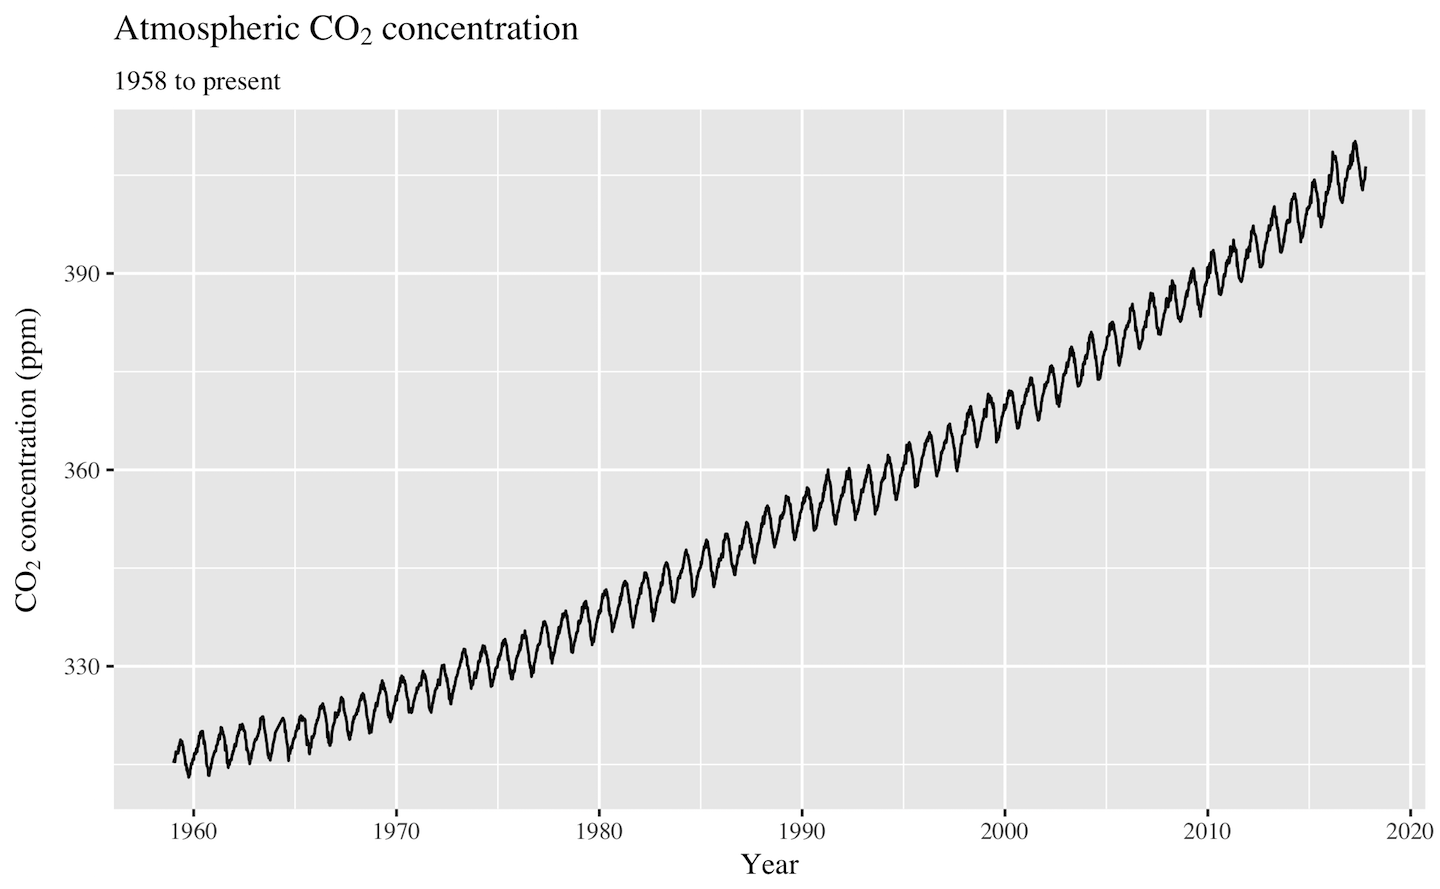
\includegraphics[width=0.8\textwidth]{mauna_loa/original_data.png}
\caption{Original data}
\end{figure}

\hypertarget{data-preprocessing}{%
\section{Data preprocessing}\label{data-preprocessing}}

Though fairly consistent, I found that a few years were missing several
values (though in 1964's case, 20 are missing). We'd want 51-53 values
per year --- usually 52, but sometimes 51 if the first measurement of
the year occurs late in the week, sometimes 53 if the first year occurs
early (as the exact number of days in a year is 365.25, we'd really
expect \textasciitilde{}52.18 weeks per year; this occasionally throws
off the discrete count). \newline

\begin{verbatim}
## [1] "Number of datapoints per year:"
\end{verbatim}

\begin{verbatim}
## 
## 1958 1959 1960 1961 1962 1963 1964 1965 1966 1967 1968 1969 1970 1971 1972 
##   25   48   53   52   48   49   31   52   49   50   52   52   52   52   53 
## 1973 1974 1975 1976 1977 1978 1979 1980 1981 1982 1983 1984 1985 1986 1987 
##   52   52   52   51   53   52   52   52   52   52   53   48   51   52   52 
## 1988 1989 1990 1991 1992 1993 1994 1995 1996 1997 1998 1999 2000 2001 2002 
##   53   52   52   52   52   52   53   52   52   52   52   52   53   52   52 
## 2003 2004 2005 2006 2007 2008 2009 2010 2011 2012 2013 2014 2015 2016 2017 
##   49   52   49   50   51   52   52   52   53   50   52   52   52   53   47
\end{verbatim}

Where I could, I interpolated missing values by taking simple averages
of the ppm values immediately neighboring them; considering the relative
simplicity of the dataset, this strategy seems innocuous enough. In a
few cases, there's a string of missing values: there, I make up the
difference in equidistant intervals (there are only ever gaps on the
side of a peak or trough, never where it seems a peak or trough is
missing, so it seems fair to assume monotonically increasing or
decreasing interpolated sequences in these cases). \newline

Here are the graphs for 1961 and 1964, respectively: the former came in
with a value for all 52 weeks, whereas the latter was missing 20 values
(this is the most extreme case; most years with missing values were only
missing 1 or 2). \newline

\begin{figure}
\centering
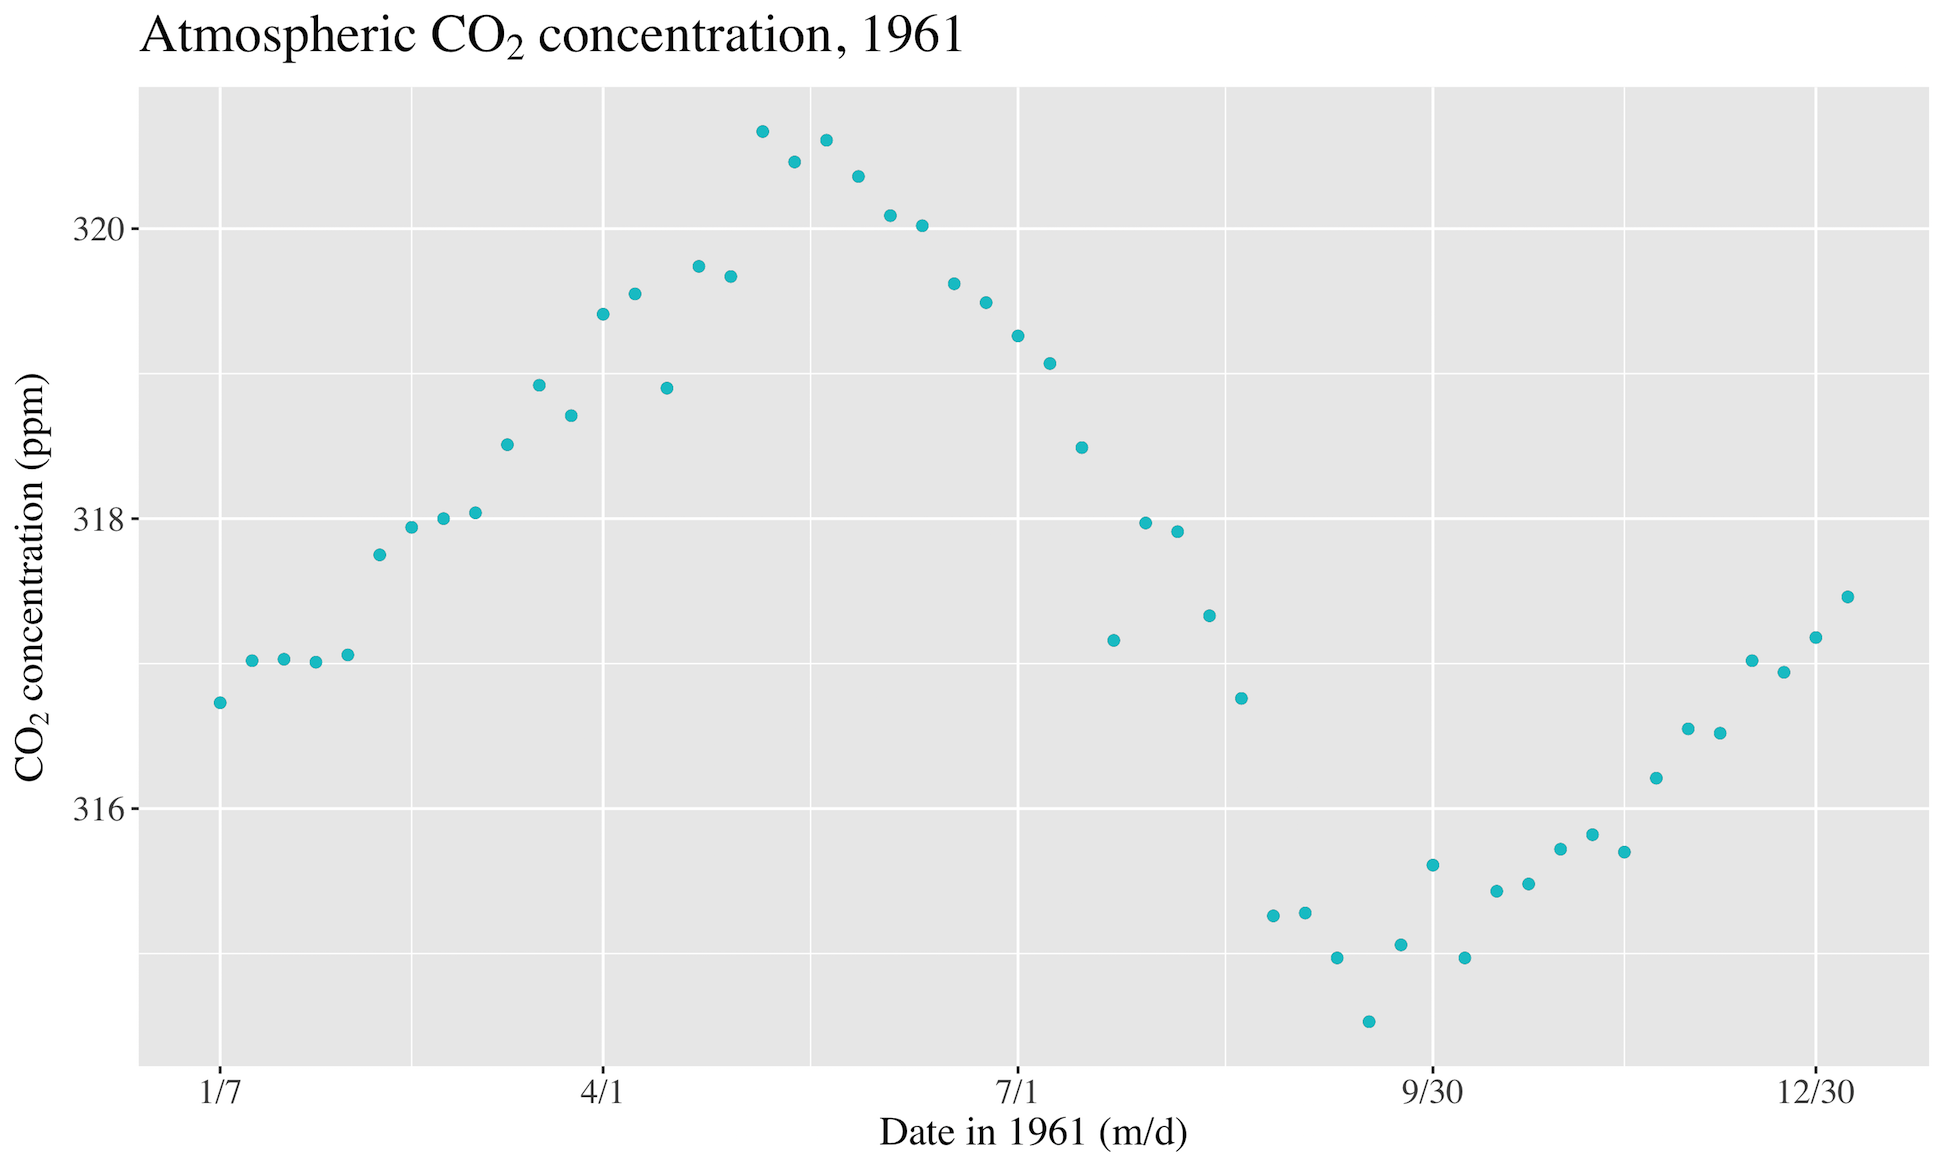
\includegraphics[width=0.7\textwidth]{mauna_loa/1961.png}
\caption{One year of data}
\end{figure}

\begin{figure}
\centering
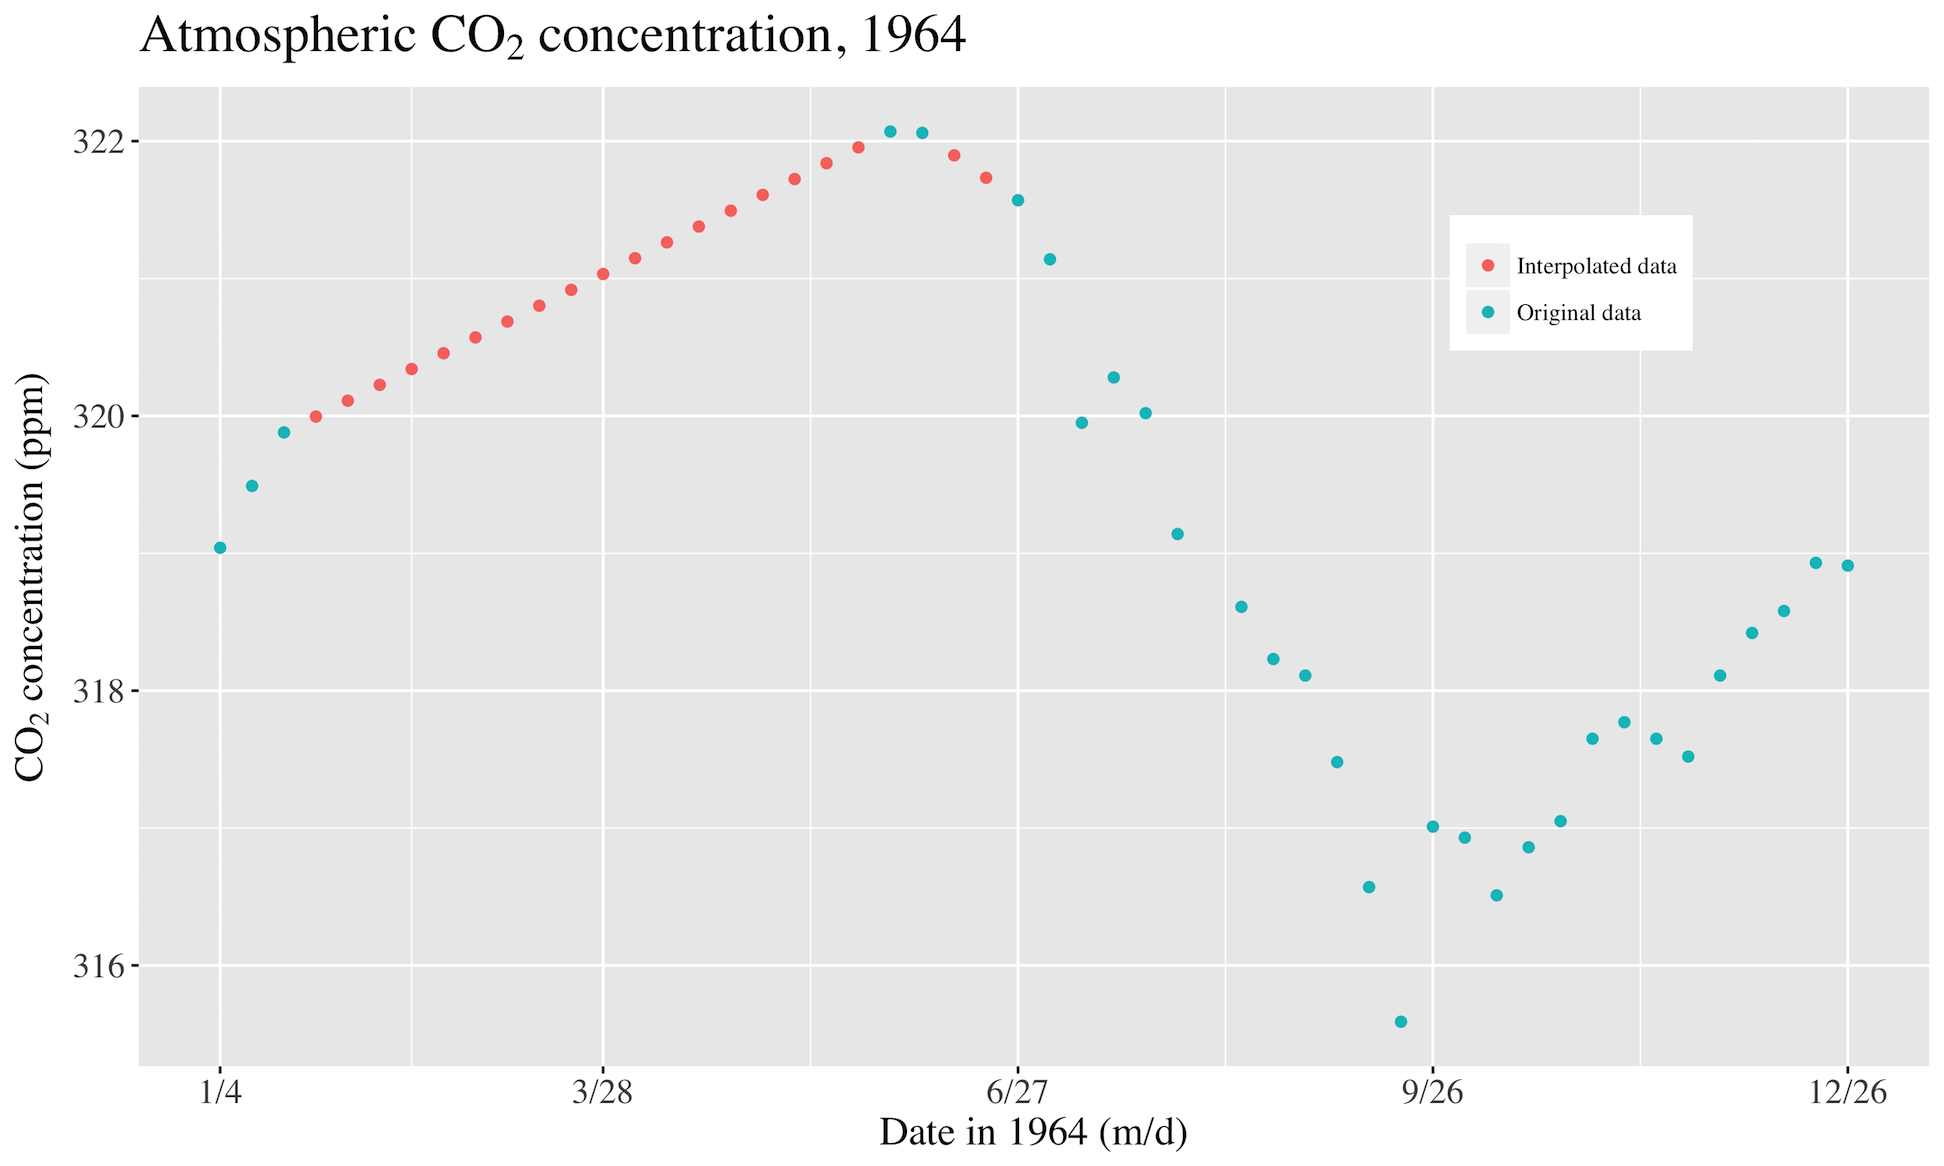
\includegraphics[width=0.7\textwidth]{mauna_loa/1964.png}
\caption{One year of data, with interpolations}
\end{figure}

I also generate new date values, at weekly intervals, to represent time
steps up until 2058, for which we'll generate forecasted ppm values.
\newline

\begin{verbatim}
## [1] "Data points per year, after interpolating and generating future dates"
\end{verbatim}

\begin{verbatim}
## 
## 1958 1959 1960 1961 1962 1963 1964 1965 1966 1967 1968 1969 1970 1971 1972 
##   25   52   53   52   52   51   51   52   52   52   52   52   52   52   53 
## 1973 1974 1975 1976 1977 1978 1979 1980 1981 1982 1983 1984 1985 1986 1987 
##   52   52   52   51   53   52   52   52   52   52   53   52   51   52   52 
## 1988 1989 1990 1991 1992 1993 1994 1995 1996 1997 1998 1999 2000 2001 2002 
##   53   52   52   52   52   52   53   52   52   52   52   52   53   52   52 
## 2003 2004 2005 2006 2007 2008 2009 2010 2011 2012 2013 2014 2015 2016 2017 
##   52   52   53   52   51   52   52   52   53   52   52   52   52   53   52 
## 2018 2019 2020 2021 2022 2023 2024 2025 2026 2027 2028 2029 2030 2031 2032 
##   52   52   52   52   53   52   52   52   52   52   53   52   52   52   52 
## 2033 2034 2035 2036 2037 2038 2039 2040 2041 2042 2043 2044 2045 2046 2047 
##   53   52   52   52   52   52   53   52   52   52   52   53   52   52   52 
## 2048 2049 2050 2051 2052 2053 2054 2055 2056 2057 2058 
##   52   52   53   52   52   52   52   52   53   52    1
\end{verbatim}

To permit models that evaluate ppm as a function of time step
\texttt{t}, I assigned integer values to each date, representing days
elapsed since the first date available in the data, \texttt{1958-03-29}:
i.e., \texttt{1958-03-29} \(\rightarrow\) \texttt{0},
\texttt{1958-04-05} (the next date, representing the CO\(_2\)
measurement taken one week after the first) \(\rightarrow\) \texttt{7},
\texttt{1958-04-12} \(\rightarrow\) \texttt{14}, etc.. I'll call these
\texttt{day} values. \newline

The range of ppm values is \texttt{313.04} to \texttt{410.18}; day
values, \texttt{0} to \texttt{21791}. To simplify the assignment of
priors for each parameter in the models, I normalized the data --- both
ppm and day values --- to reside in the interval \([0, 1]\). \newline

Finally, I separate the data (not including generated future timesteps)
into a training and test set by an 80/20 split. \newline

\hypertarget{model-development-and-prior-selection}{%
\section{Model development and prior
selection}\label{model-development-and-prior-selection}}

I begin with the assumption that an appropriate model can be decomposed
into a long-term trend to account for general trajectory, a seasonal
trend to account for peaks during northern hemisphere winters and
troughs during northern hemisphere summers (see \emph{CO\(_2\)
seasonality pattern} below), and an noise component. \newline

\begin{figure}
\centering
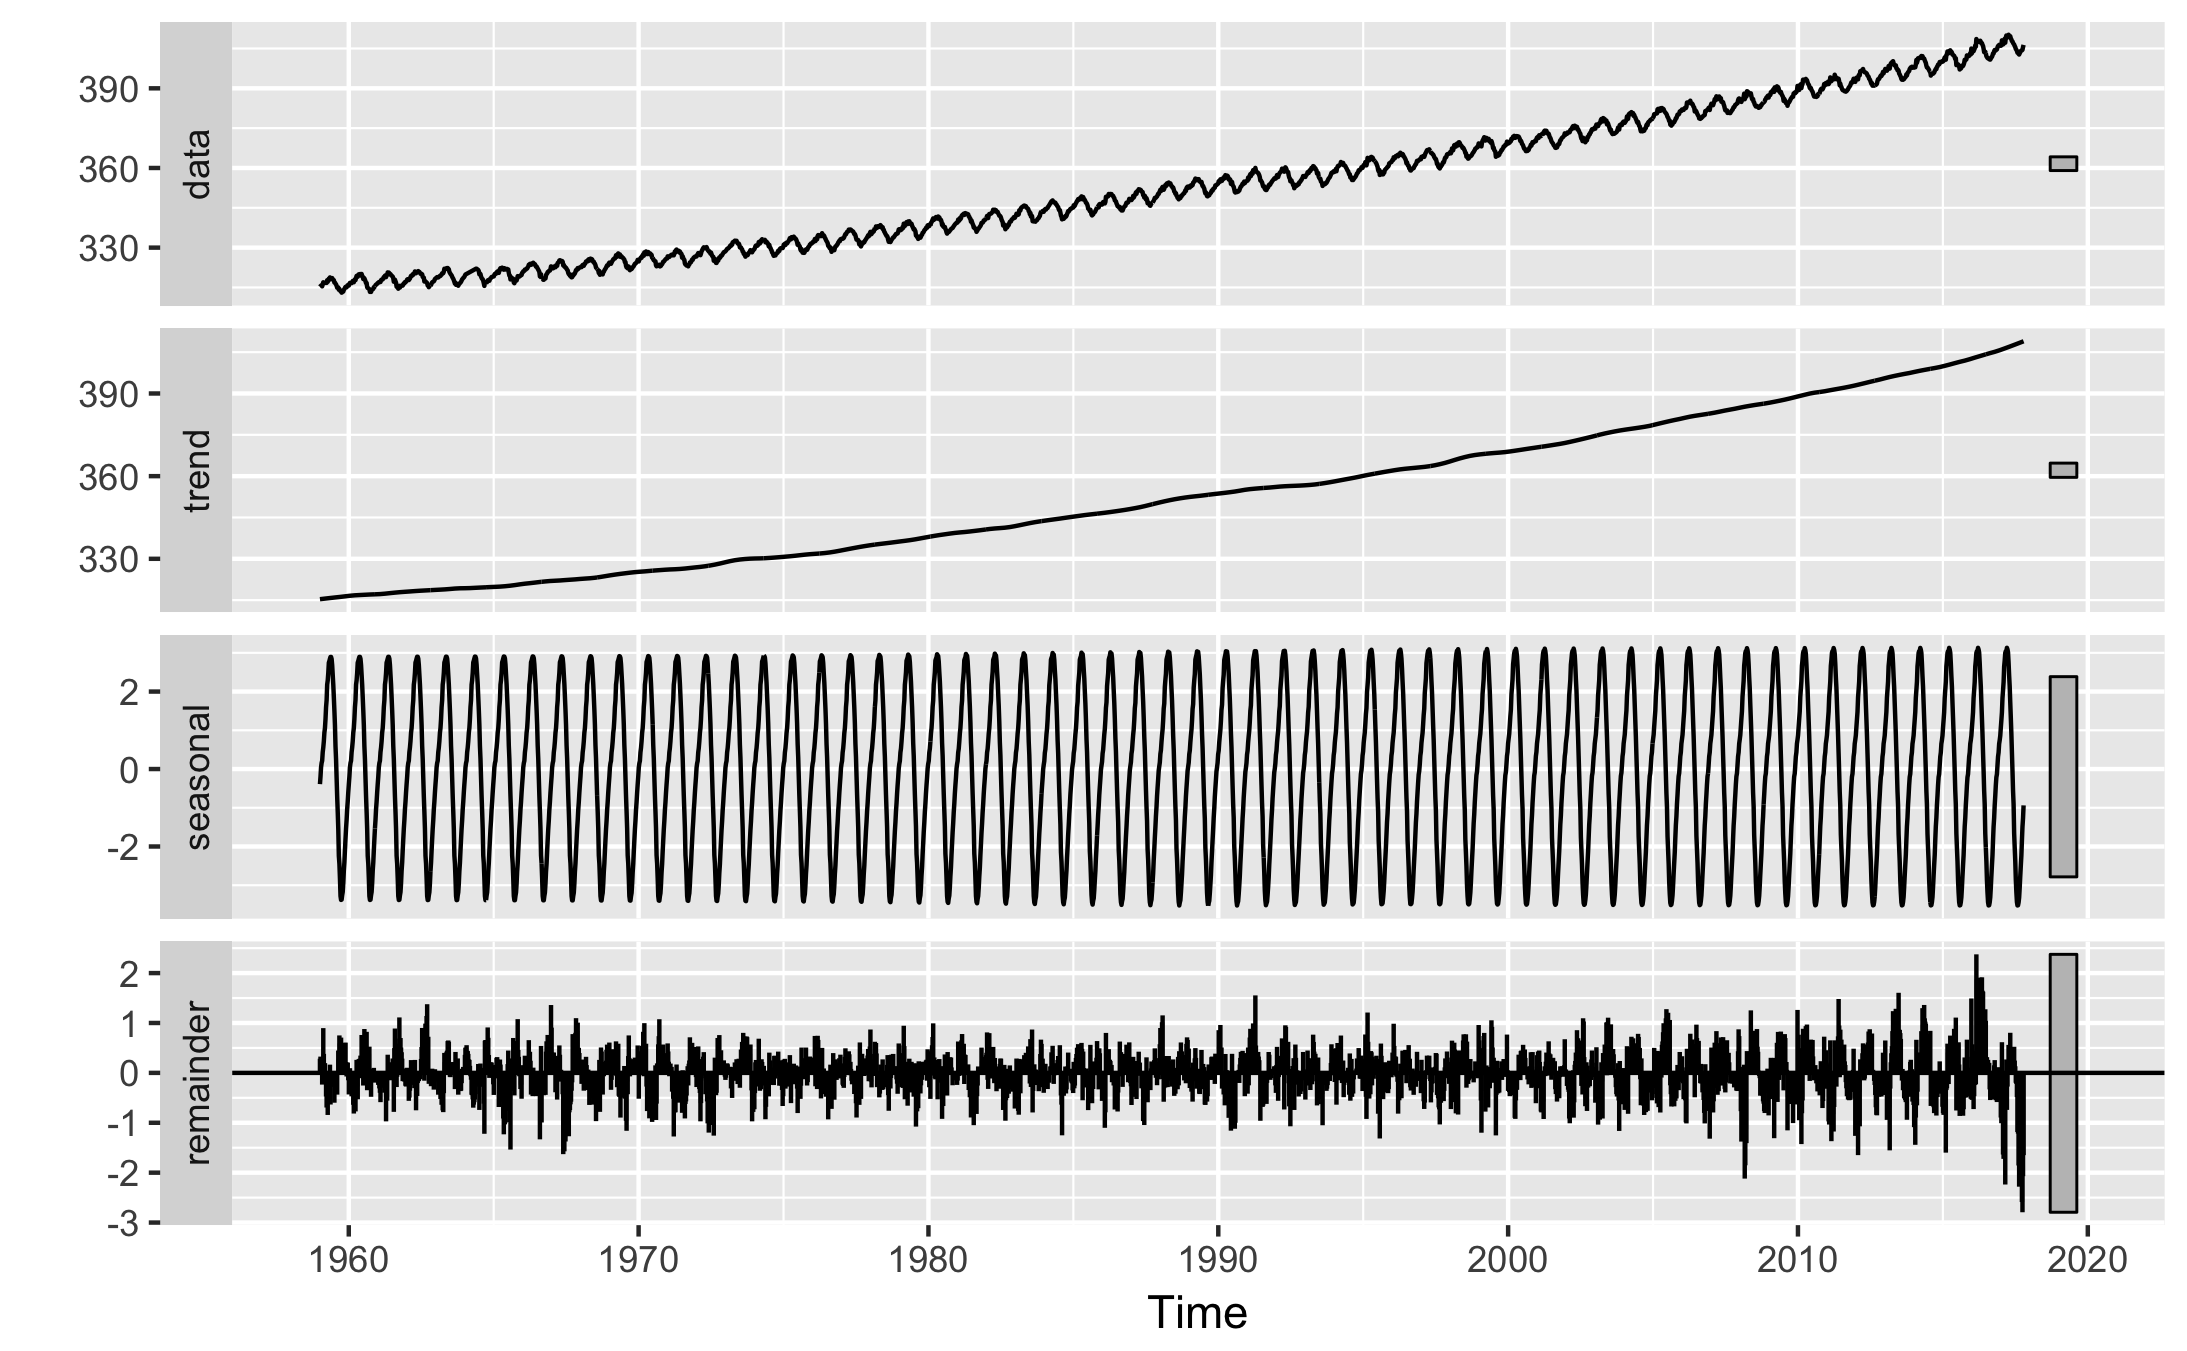
\includegraphics[width=0.8\textwidth]{mauna_loa/components.png}
\caption{Decompositions}
\end{figure}

\hypertarget{long-term-trend}{%
\subsection{Long-term trend}\label{long-term-trend}}

By smoothing the time series by taking a moving average with length =
seasonal span, we find something other than a linear long-term
trend.\newline

\begin{figure}
\centering
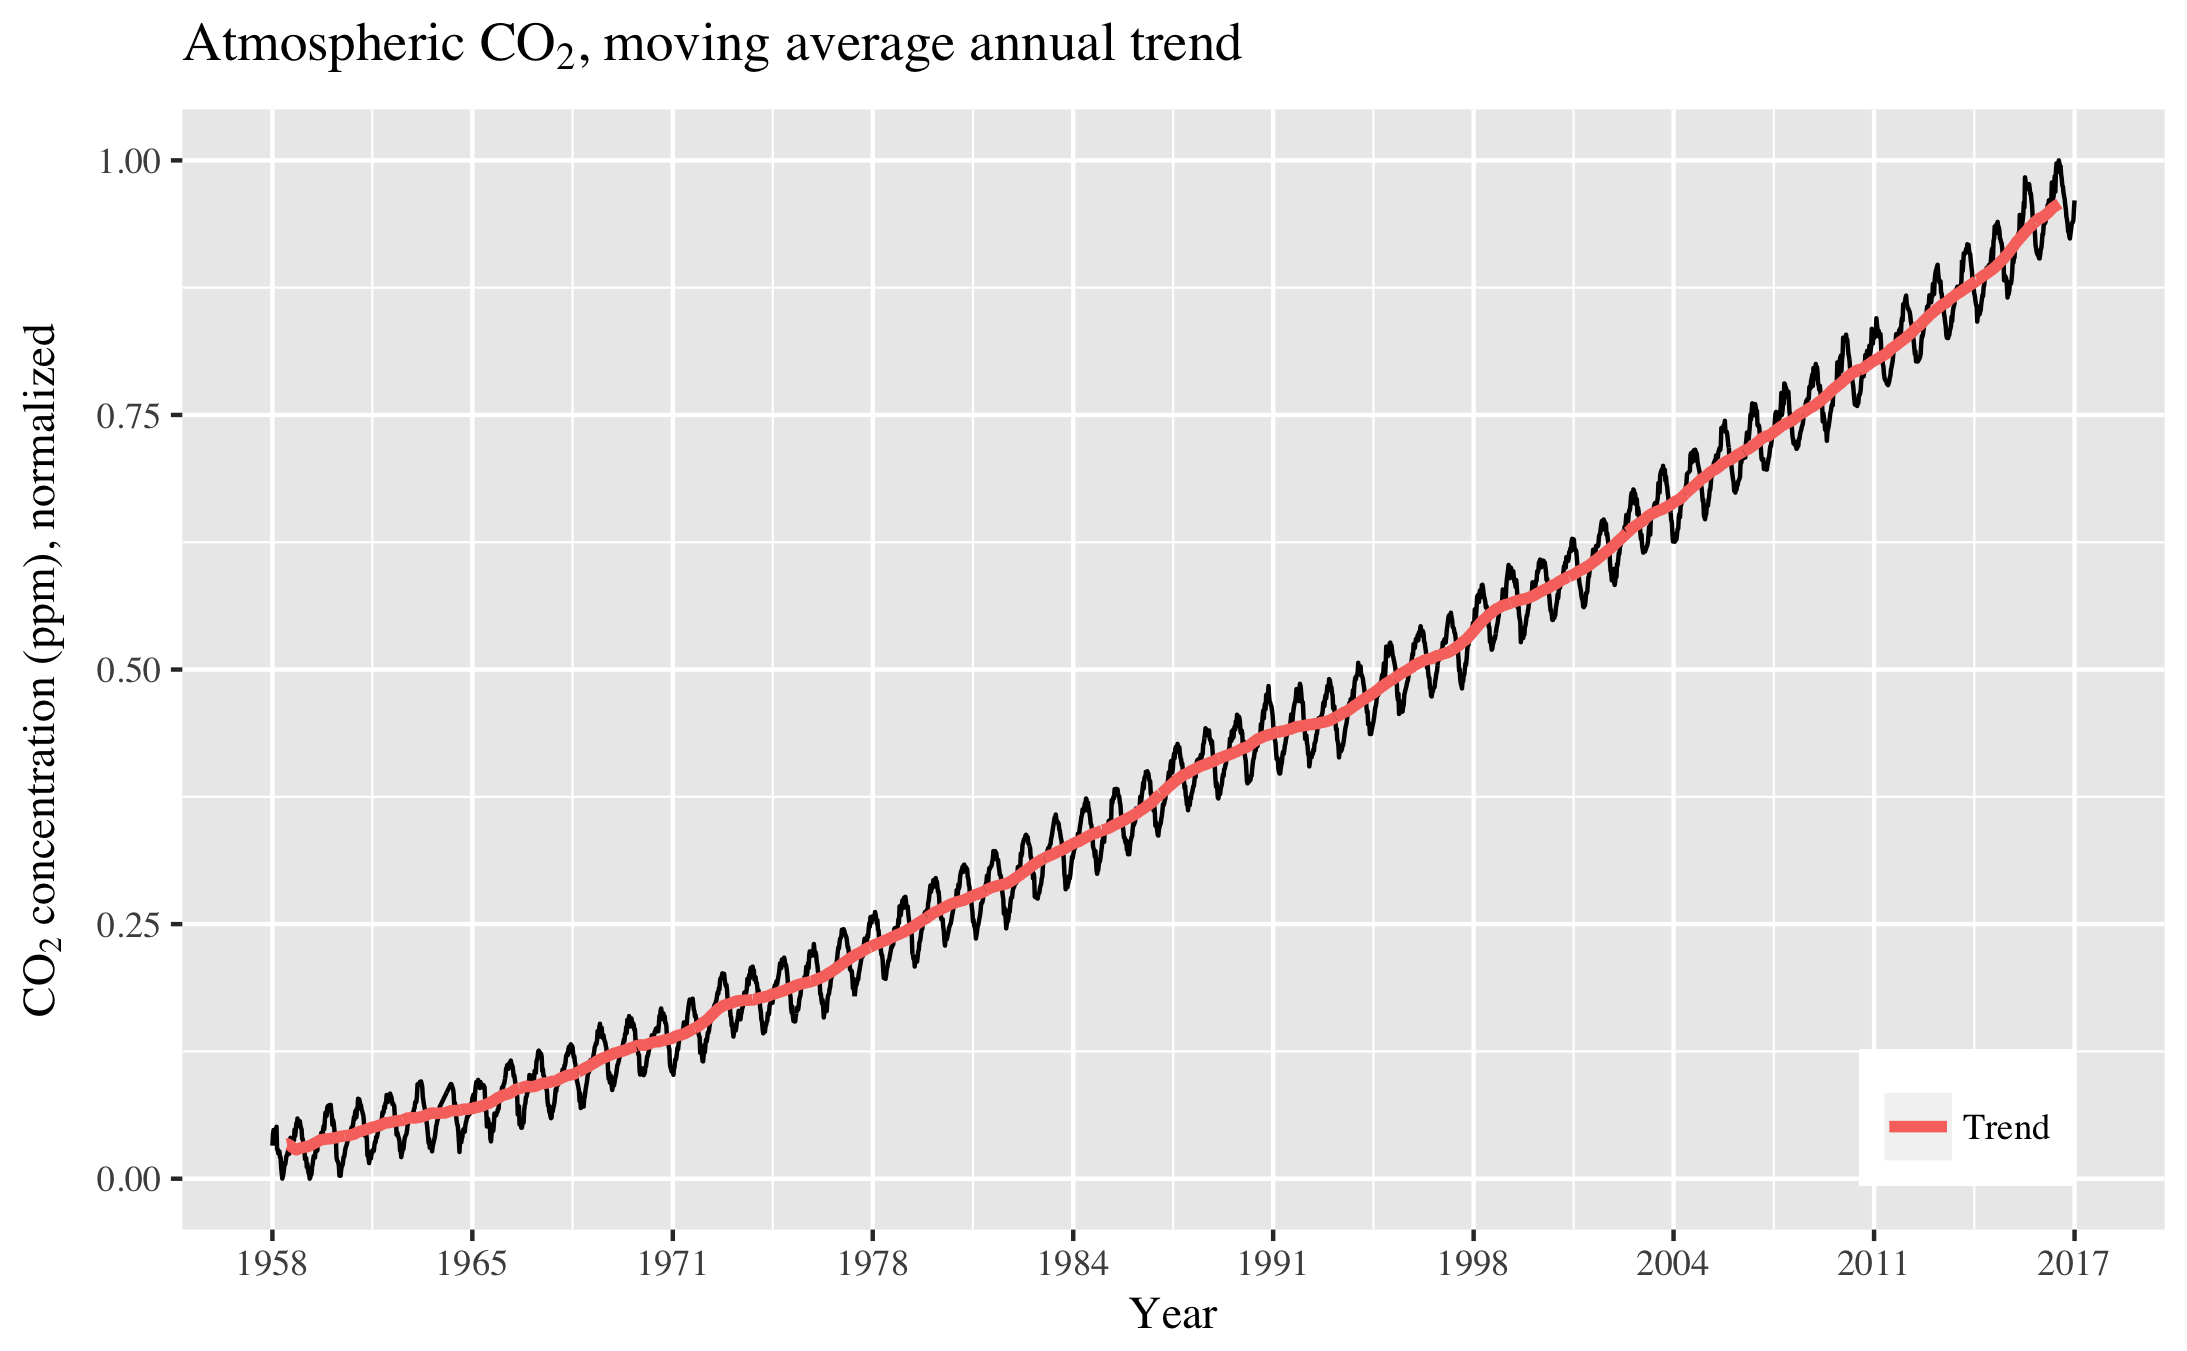
\includegraphics[width=0.6\textwidth]{mauna_loa/moving_averages.png}
\caption{Moving averages}
\end{figure}

Just to check them out, I fitting second to fourth order polynomials
with \texttt{R}'s linear modeling functionality. All shared an R\(^2\)
score exceeding 0.98.\newline

\begin{figure}
\centering
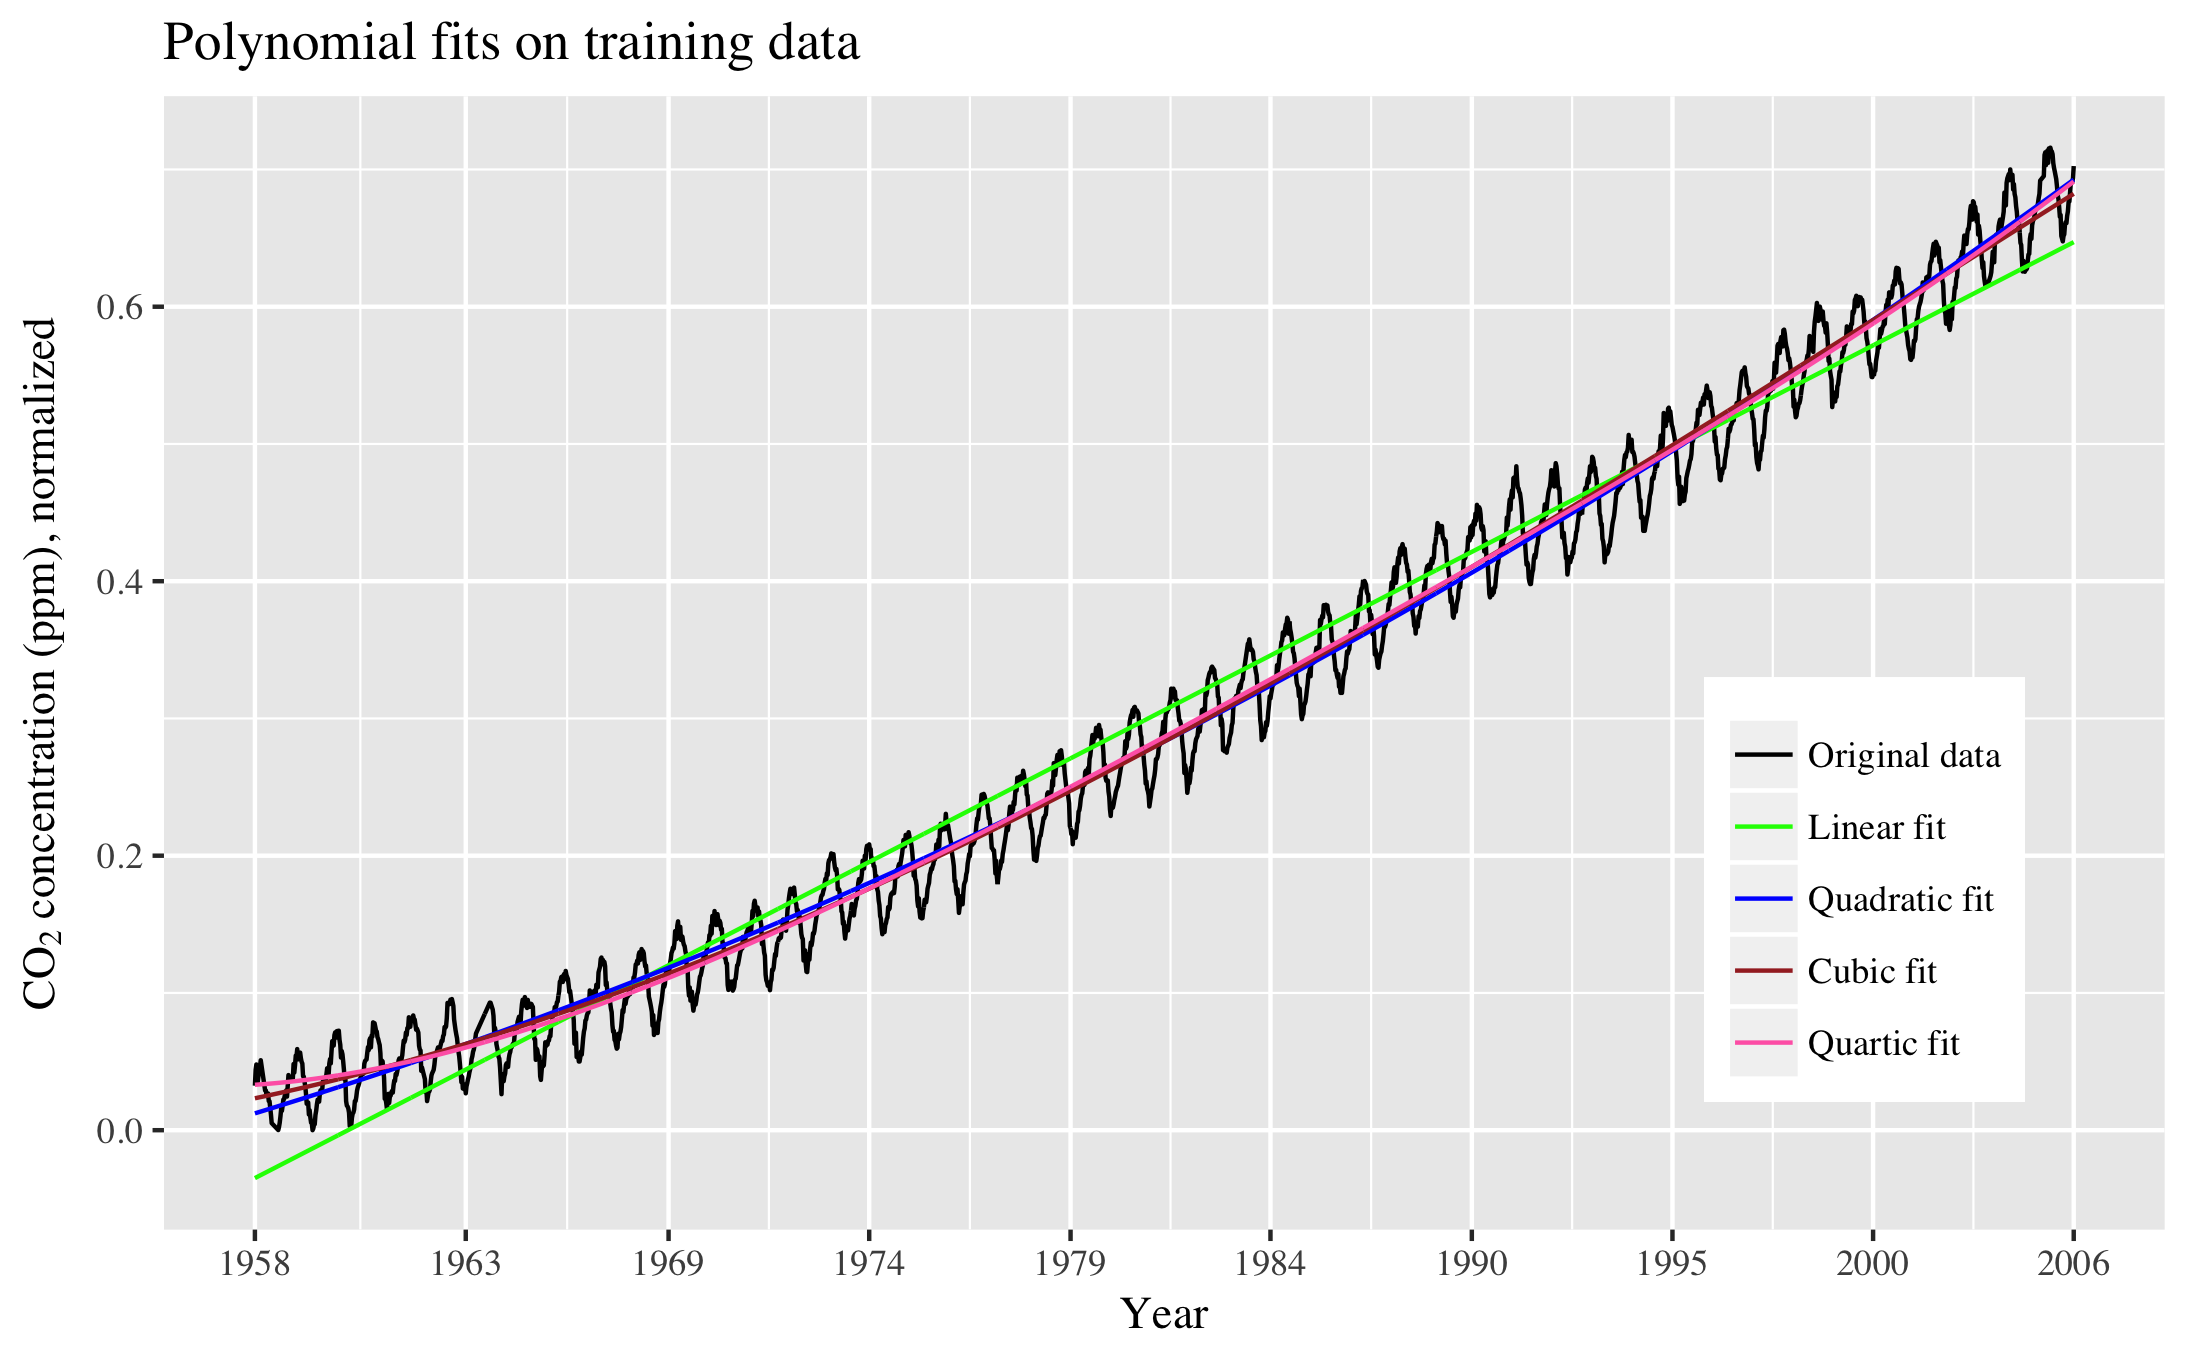
\includegraphics[width=0.6\textwidth]{mauna_loa/polynomial_fits.png}
\caption{Polynomial fits}
\end{figure}

I tried several models for the long-term component, including 2nd order
polynomial, 3rd order polynomial, and exponential functions. I found
that the 3rd order polynomial (i.e., cubic) model failed to outperform
the 2nd order (i.e., quadratic) one; I don't include analysis of a cubic
model in this report.\newline

\hypertarget{seasonal-model}{%
\subsection{Seasonal model}\label{seasonal-model}}

We see that CO\(_2\) peaks in May of each year, and hits its low in
September. Why does the peak occur so late in the spring? Presumably,
the boreal and temperature forests of the world's largest forested
landmass --- Siberia --- don't swing back into full photosynthetic
production until then.\newline

\begin{figure}
\centering
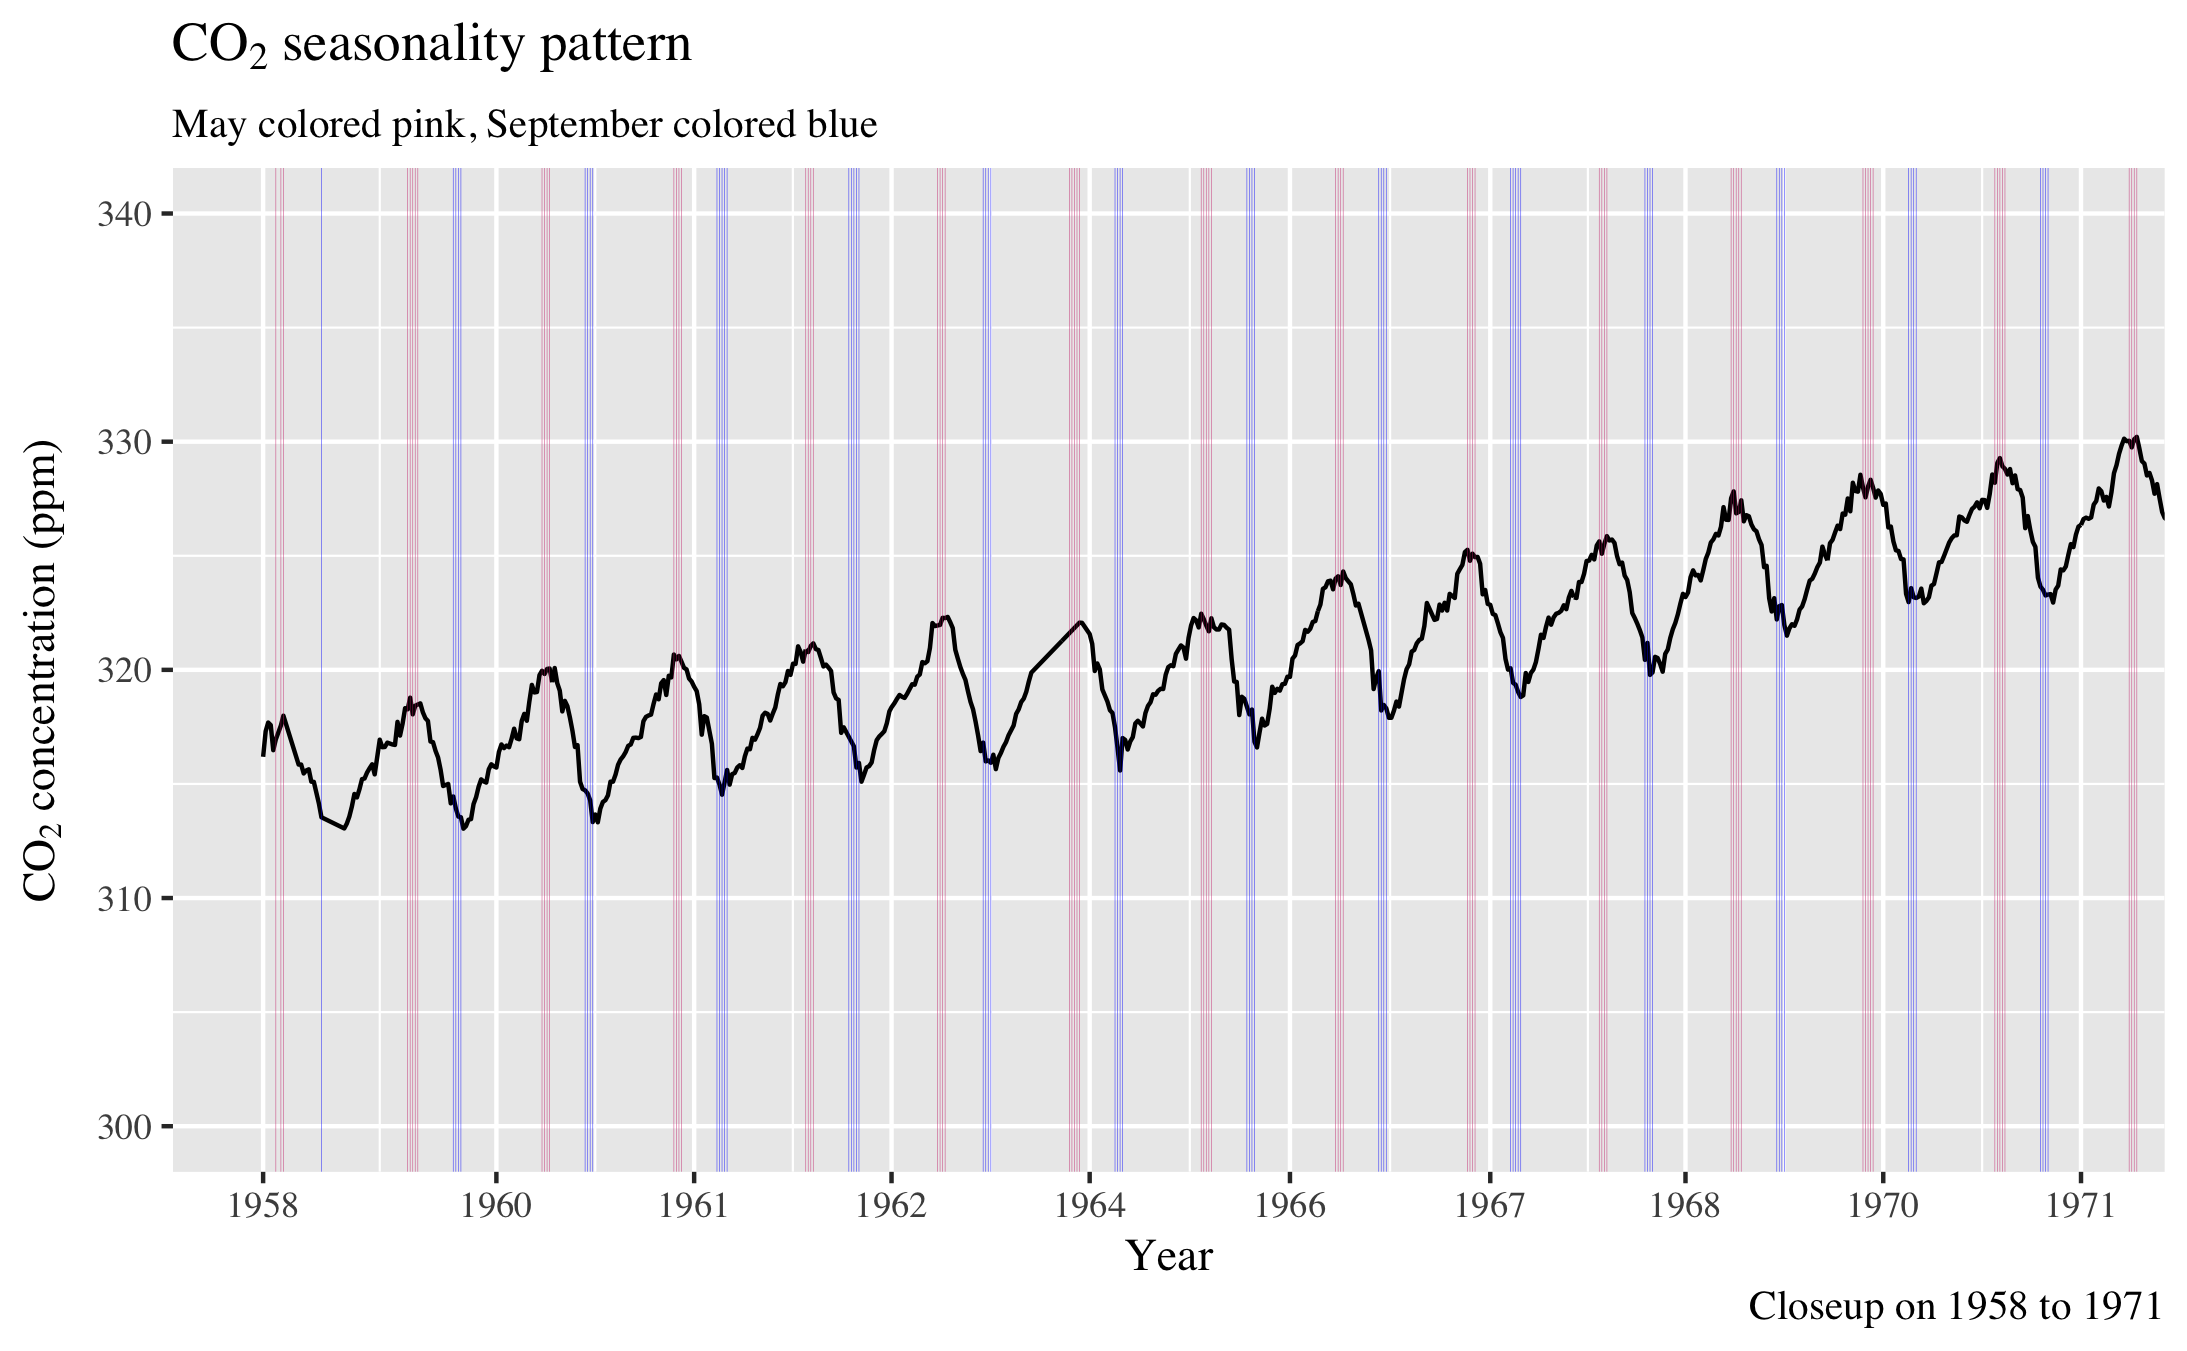
\includegraphics[width=0.7\textwidth]{mauna_loa/peaks_troughs.png}
\caption{Seasonal peaks and troughs}
\end{figure}

If we subtract the long-term trend from the data, we find a very
consistent seasonal trend (see next page). The following graph shows the
data plotted against the seasons in each year. We see what looks like
slowly increasing distances between each year over time, and affirm the
uniformity of peaks in May (around week 21) and troughs in September
(around week 40). \newline

\begin{figure}
\centering
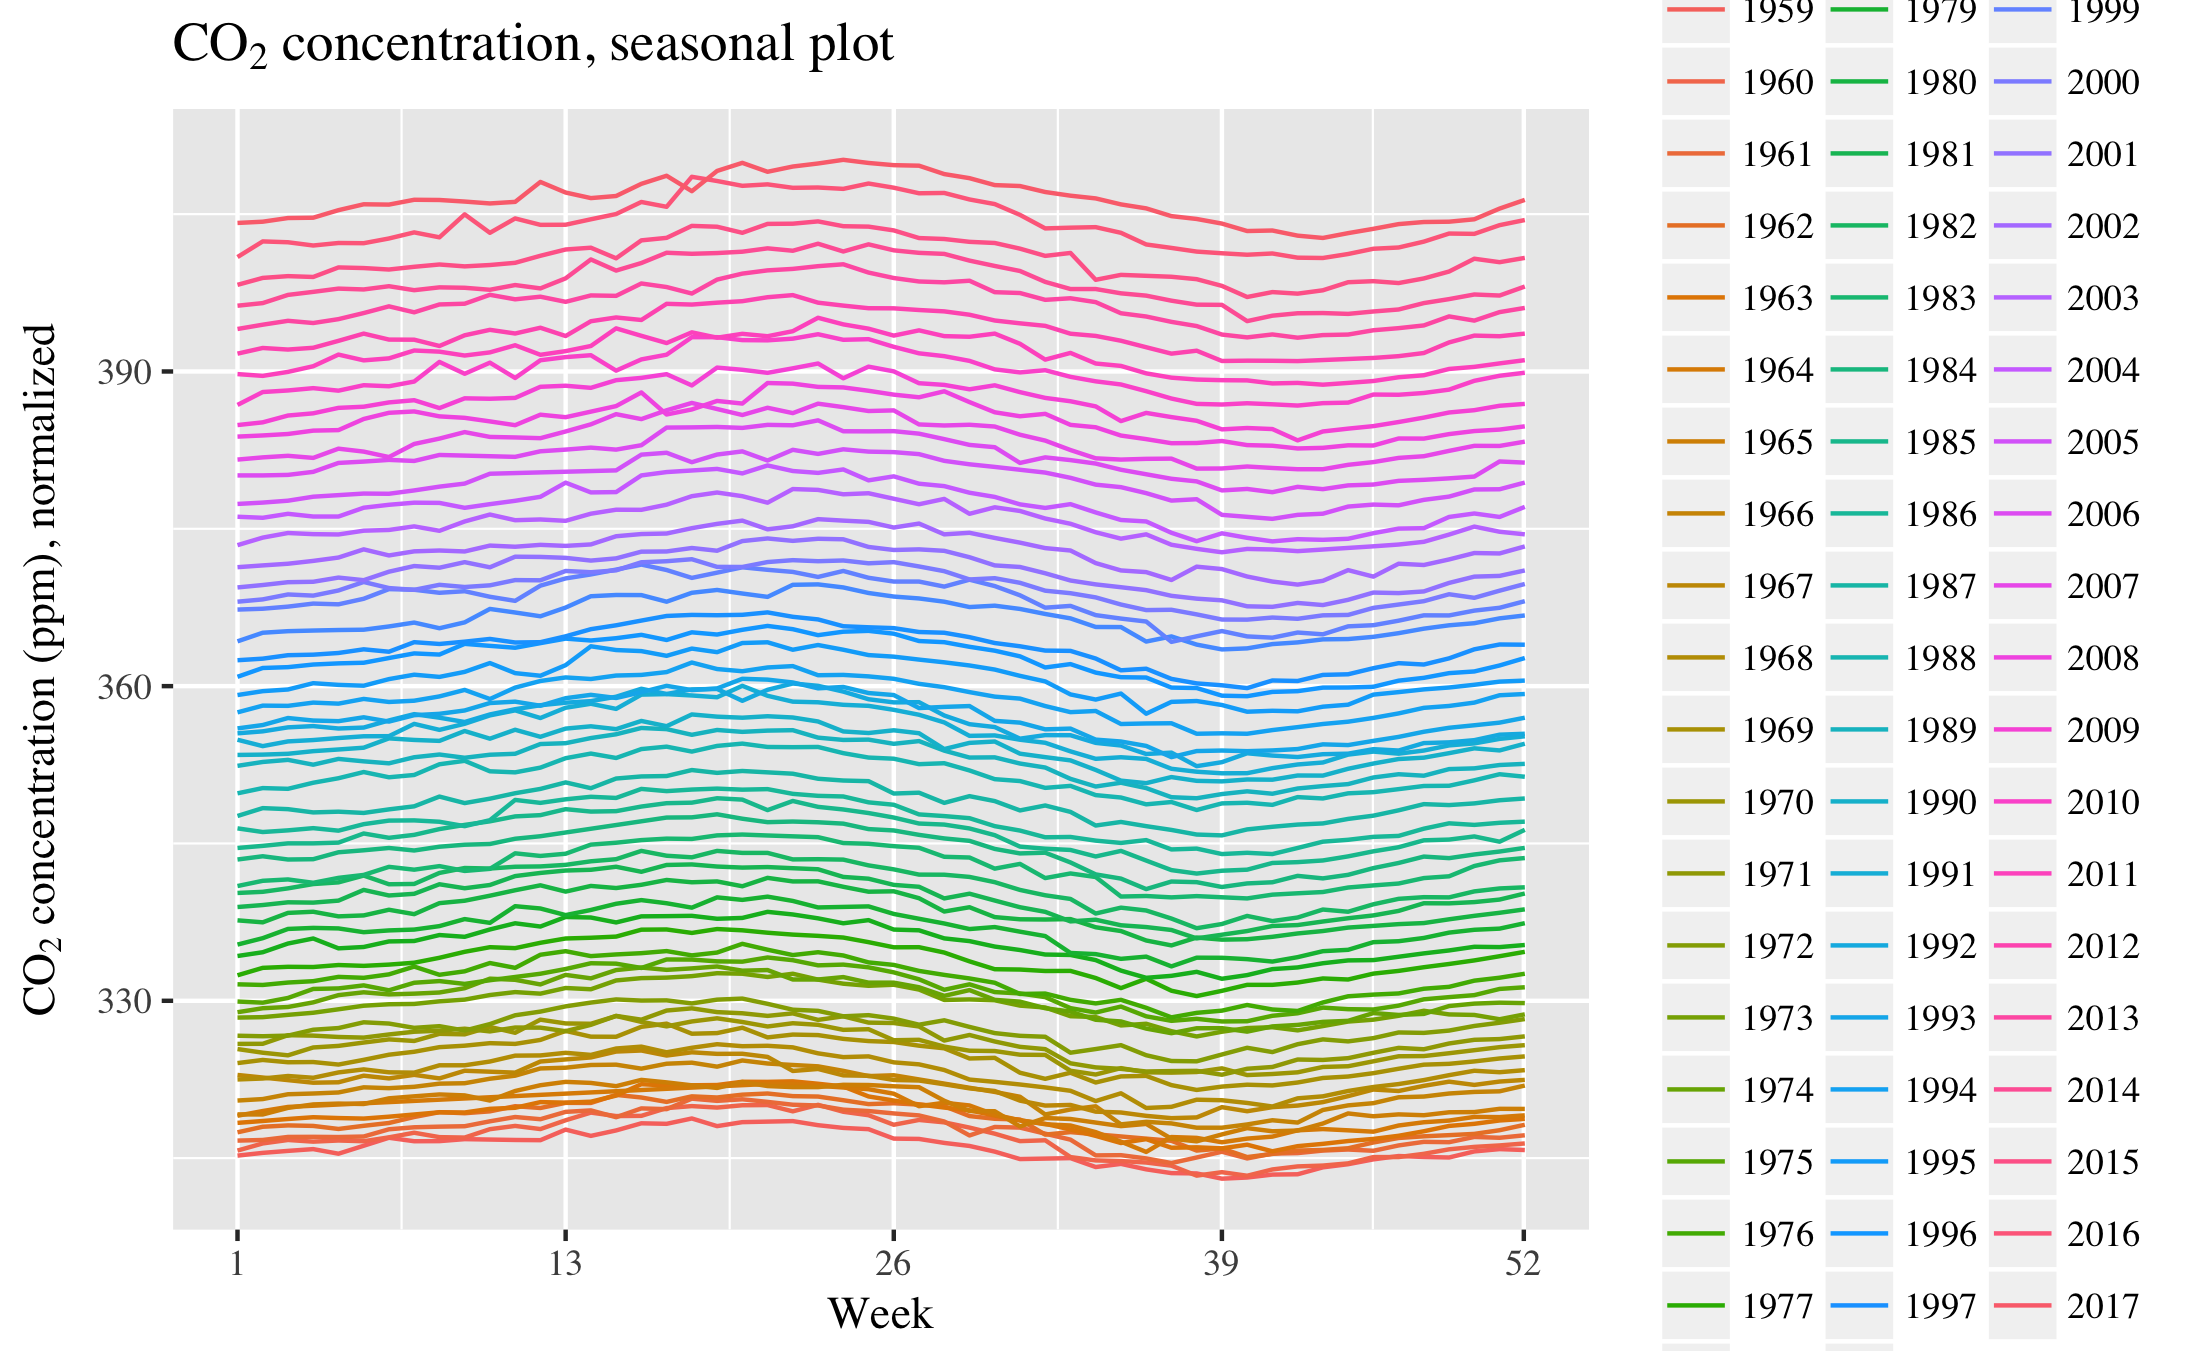
\includegraphics[width=0.7\textwidth]{mauna_loa/seasonal_plot.png}
\caption{Seasonal trend, by year}
\end{figure}

\begin{figure}
\centering
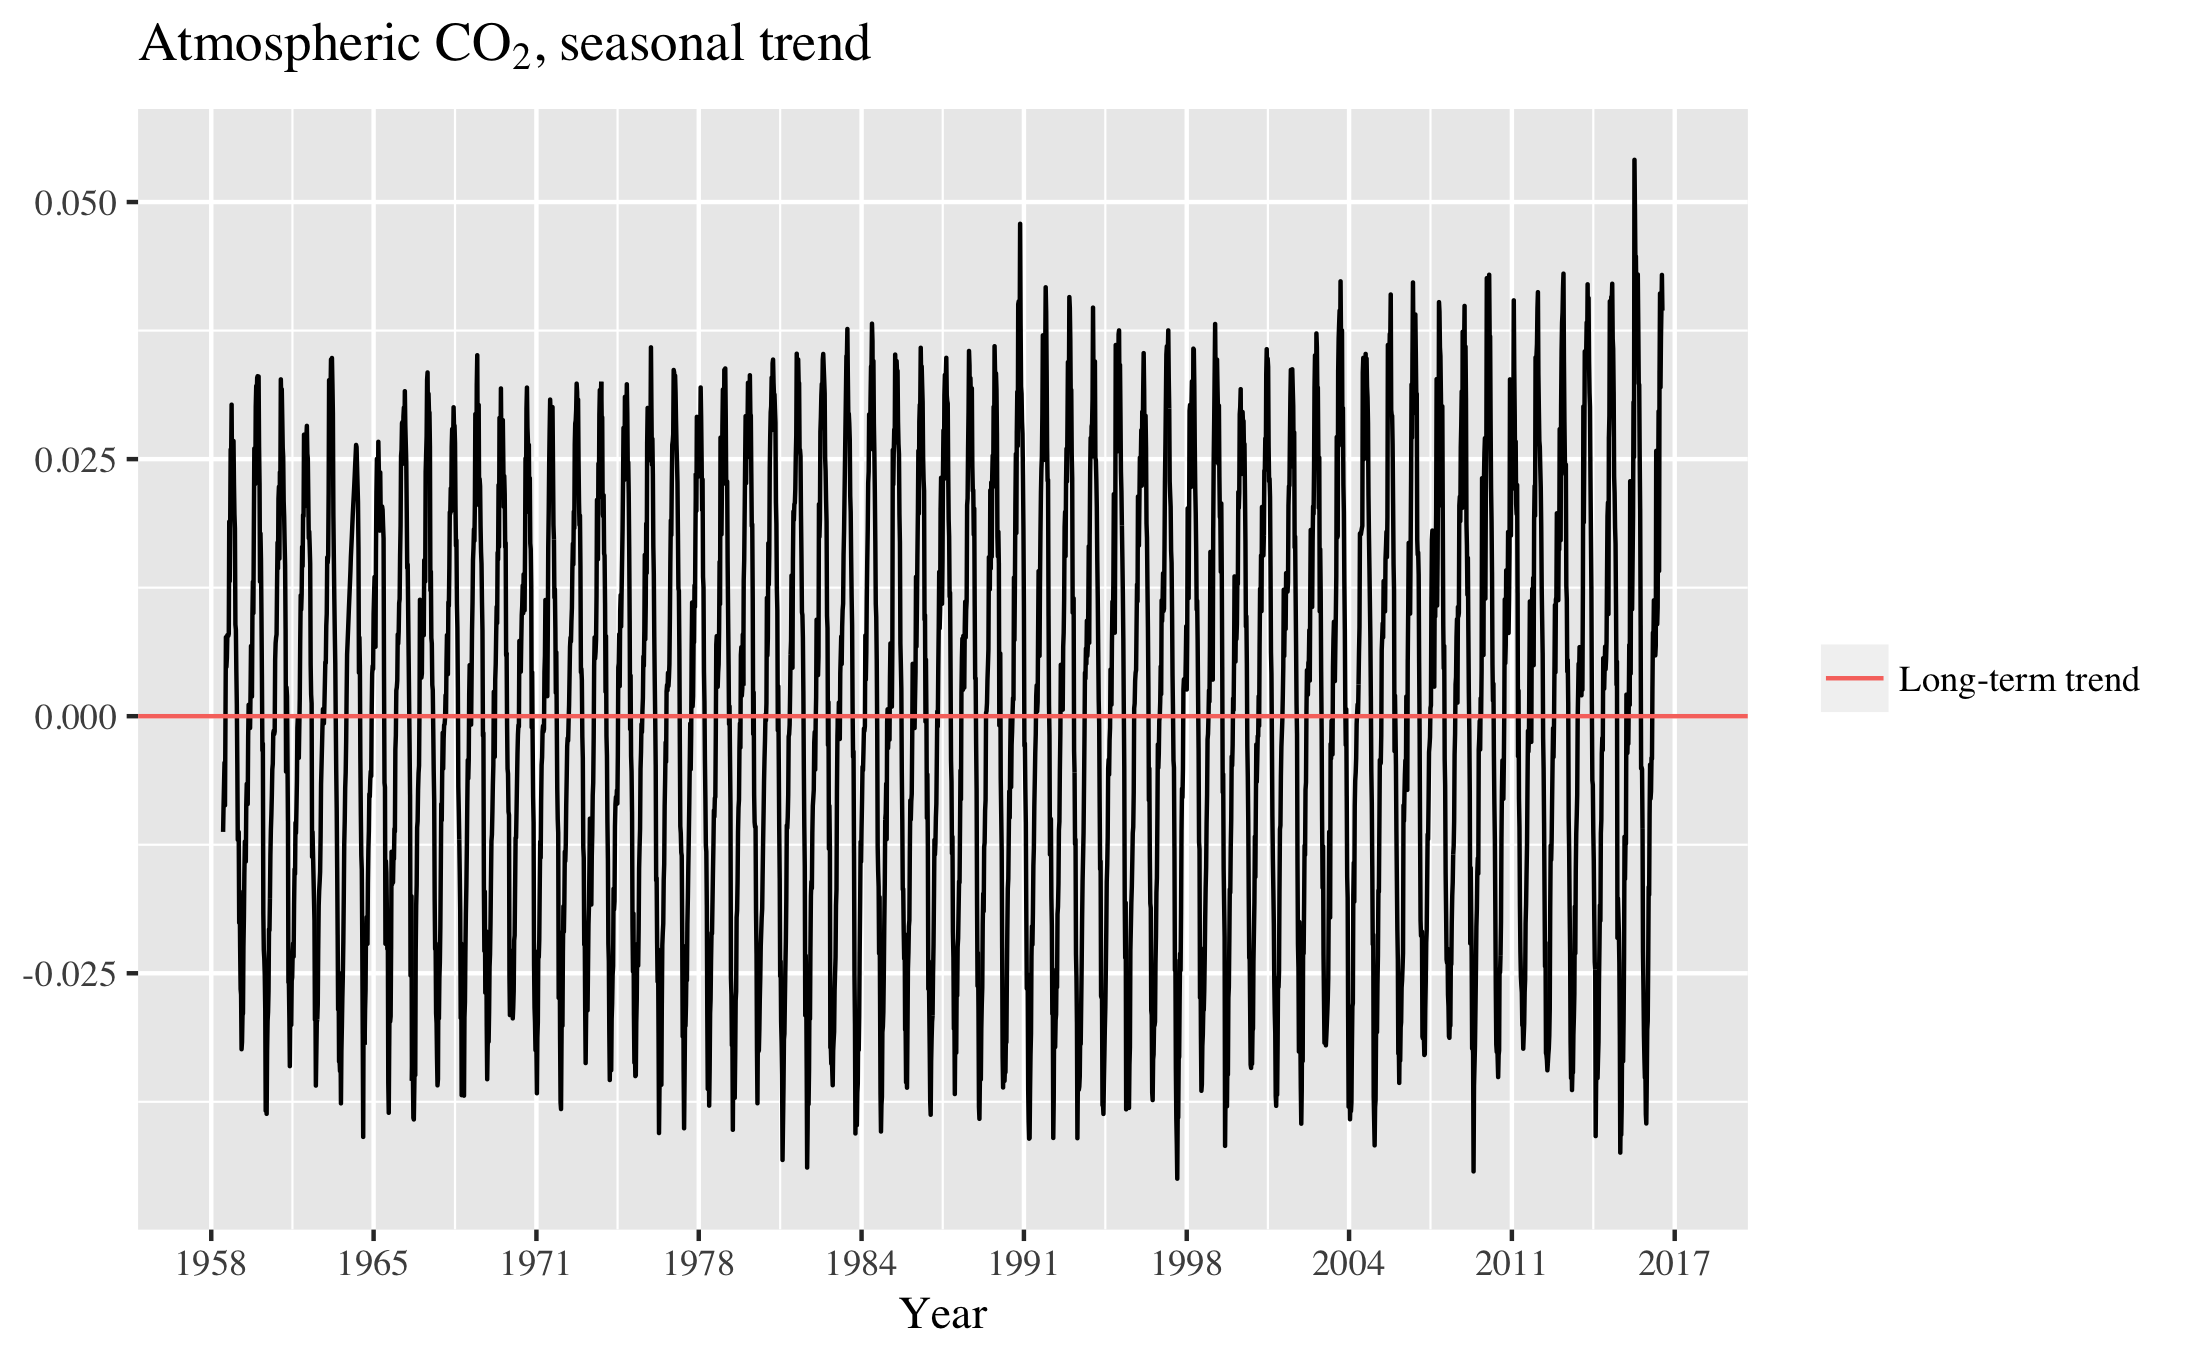
\includegraphics[width=0.7\textwidth]{mauna_loa/seasonal_trend.png}
\caption{Seasonal trend, over years}
\end{figure}

I elect to move forward with a trigonometric periodic function to model
seasonality (I'll use a cosine function), but this assumption may be
limiting: the seasonal trend above seems to indicate that seasonal peaks
are actually getting more extreme over time (interestingly, troughs seem
consistent), and the static amplitude of a cosine function will fail to
capture that.\newline

\hypertarget{noise-model}{%
\subsection{Noise model}\label{noise-model}}

I make the assumption of normally distributed noise. This is an easy
assumption to make, and further work might try a Gamma distribution.

\hypertarget{final-models}{%
\section{Final models}\label{final-models}}

I propose the following two models. \newline

The \textbf{quadratic model} entails the likelihood function

\[p(ppm_i\ |\ c_0, c_1, c_2, A, \phi, \sigma ) = N(c_0 + c_{1}t_i + c_{2}t_{i}^2 + A(cos(\frac{21791(2\pi t_i)}{365.25} + \phi), \sigma)\]

where CO\(_2\) concentration at time \(t_i\), \(ppm_i\), is normally
distributed around a quadratic trend parameterized by \(c_0\), \(c_1\),
and \(c_2\), a seasonal component parameterized by amplitude \(A\) and
phase \(\phi\), and with a standard deviation of \(\sigma\). Note that
we divide the period of the seasonal trend by 365.25 --- the number of
days in the year --- to describe the number of days in each period, and
that we multiply is by 21,791 --- the number of days, total, that
comprise the dataset --- to account for the normalization on the
interval \([0, 1]\).\newline

The \textbf{exponential model} entails the likelihood function \newline

\[p(ppm_i\ |\ c_0, c_1, c_2, A, \phi, \sigma ) = N(c_0 + c_{1}c_{2}^{t_i} + A(cos(\frac{21791(2\pi t_i)}{365.25} + \phi), \sigma)\]
where, instead of a quadratic long-term trend, the term
\(c_1 c_2^{t_i}\) introduces an exponential function. Otherwise, the
models are similar.

\hypertarget{prior-selection}{%
\section{Prior selection}\label{prior-selection}}

\hypertarget{quadratic-model-priors}{%
\subsection{Quadratic model priors}\label{quadratic-model-priors}}

In order to arrive at the quadratic model's priors, I considered the
intervals in which I thought I could reasonably expect each parameter to
live. With \emph{ppm} values bound between 0 and 1, I'd start with hard
bounds on \(\sigma\), the error term, and \(A\), the amplitude of the
seasonal component. At the very least, all of these would have to be
bound on \([0, 1]\) themselves (I arrive at more specific priors
shortly).\newline

I assign the phase parameter, \(\phi\), a Normal prior
\(N(0, \frac{\pi}{2})\), suggesting a lower bound of \(-\pi\) and upper
bound of \(\pi\) (I tried a uniform prior over this interval initially,
but ran into sampling errors; the Normal prior worked decently). As for
\(c_1\) and \(c_2\), the trend coefficients, I have no \emph{a priori}
reason to assume positive values (though they obviously are). In the
interest of rigor, I don't require that they be positive. The intercept
term, \(c_0\), should be somewhere around 0. I give them all Normal
priors, and for a sanity check, I sampled from the Normals that I
hypothesized might define them:\newline

\[p(c_0) \sim N(0.02, 0.01)\] \[p(c_1) \sim N(0.45, 0.10)\]
\[p(c_2) \sim N(0.50, 0.10)\]\newline

They seem reasonable:

\begin{figure}
\centering
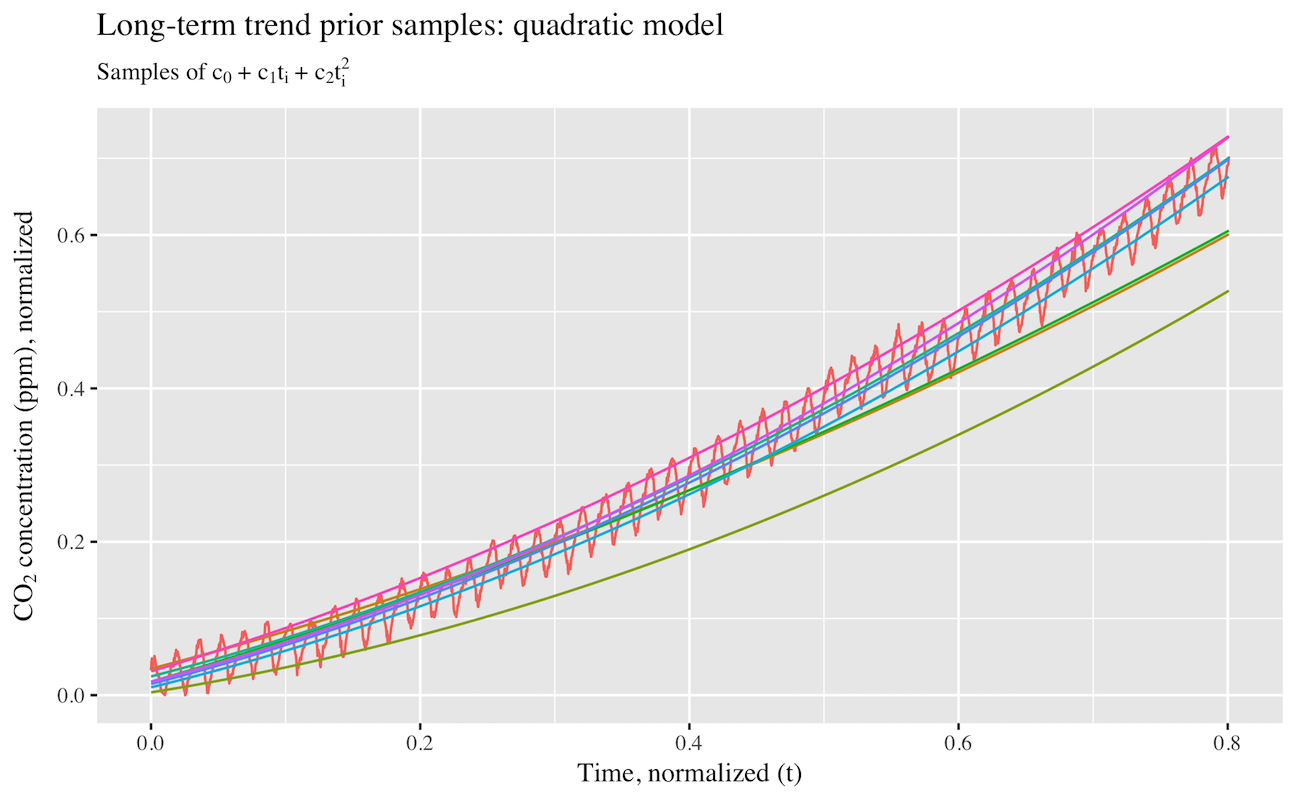
\includegraphics[width=0.7\textwidth]{mauna_loa/quad_prior_samples.png}
\caption{Quadratic model prior samples}
\end{figure}

I knew that \(A\) and \(\sigma\), the amplitude and noise parameters,
would necessarily be positive. Therefore, I transform these parameters
in \texttt{Stan} exponentially to require them to be positive (I could
explicitly require them to have a lower bound of 0, but to do this could
interfere with the quality of Stan's sampling). I assumed that \(A\)
might exist on \([0.01, 0.1]\), so I arrived at a suitable Normal prior
like so:\newline

\[ \mu_A = \frac{\ln(0.01) + \ln(0.1)}{0.2} \approx -3.45 \] and

\[ \sigma_A = \frac{\ln(0.1) - (-3.45)}{2} \approx 0.58 \] Thus, I
arrive at a log transformed prior \(p(A) \sim N(-3.45, 0.58).\) Assuming
that \(\sigma\) might sit on \([0.001, 0.05],\) and following a similar
procedure, I arrive at a prior \[ p(\sigma) \sim N(-4.95, 0.98). \]

\hypertarget{exponential-model-priors}{%
\subsection{Exponential model priors}\label{exponential-model-priors}}

I selected this latter models' prior transformations in more of an
ad-hoc fashion: I tried a few things experimentally to see what would
yield the best results. \(A\), \(\phi\), and \(\sigma\) stay the same.
However, I handle the trend coefficients --- \(c_0, c_1,\) and \(c_2\)
--- differently. Out of curiosity, I tranformed \(c_0\) with a \(tanh\)
function, to bound it to \([-1, 1]\), which I found worked adequately.
Without requiring \(c_1\) and \(c_2\) to be positive, I found suboptimal
results: I do, in this case, transform them with a sigmoid and
exponential function, respectively.\newline

Manually, I tried sampling these parameters from different Normal priors
until I found a grouping that looked appropriate (perhaps not a very
scientific method, but who's a purist here?):

\[p(c_0) \sim N(-0.7, 0.01)\] \[p(c_1) \sim N(0.4, 0.05)\]
\[p(c_2) \sim N(0.95, 0.05)\]

\begin{figure}
\centering
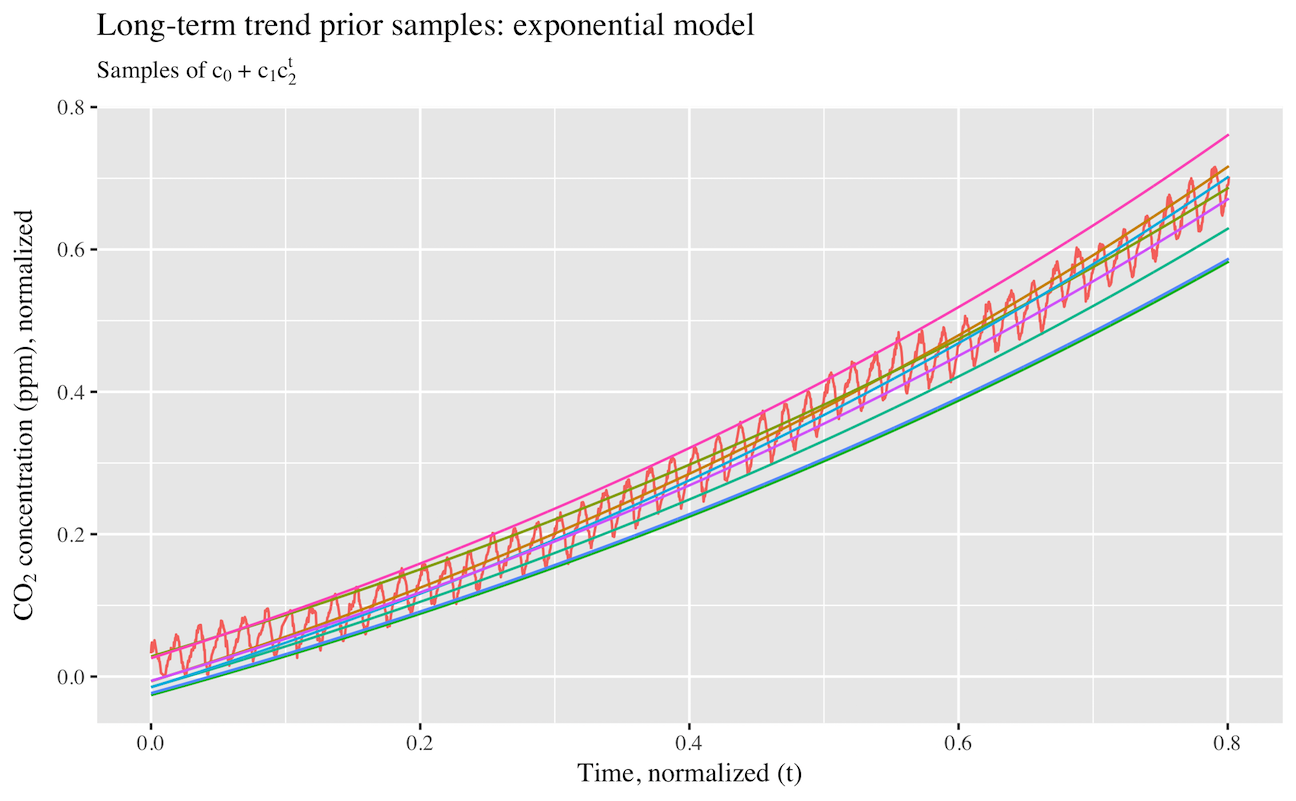
\includegraphics[width=0.7\textwidth]{mauna_loa/exp_prior_samples.png}
\caption{Exponential model prior samples}
\end{figure}

So ultimately, we arrive at the following two model proposals:

\begin{figure}
\centering
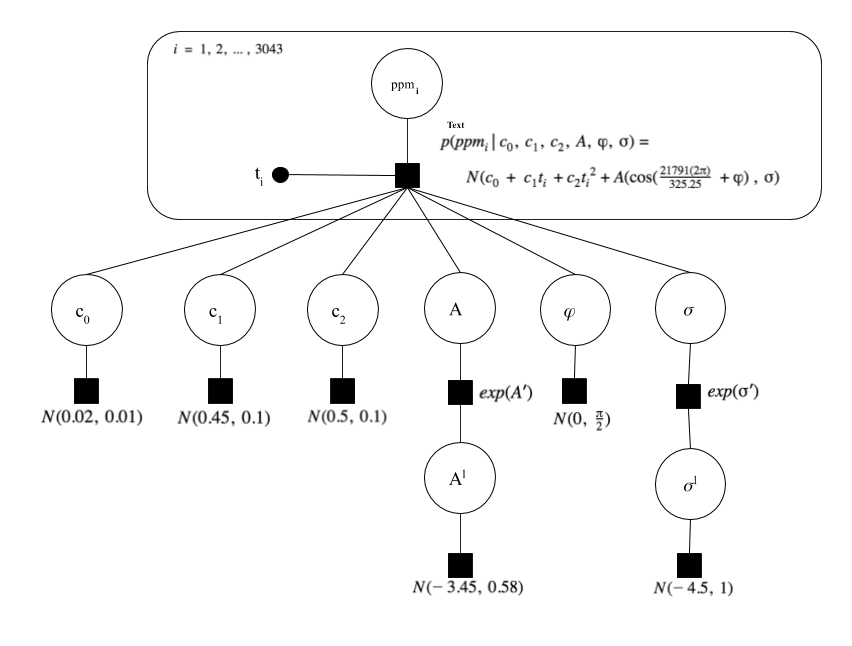
\includegraphics[width=0.8\textwidth]{mauna_loa/quadratic_graph.png}
\caption{Quadratic likelihood graphical model.}
\end{figure}

\begin{figure}
\centering
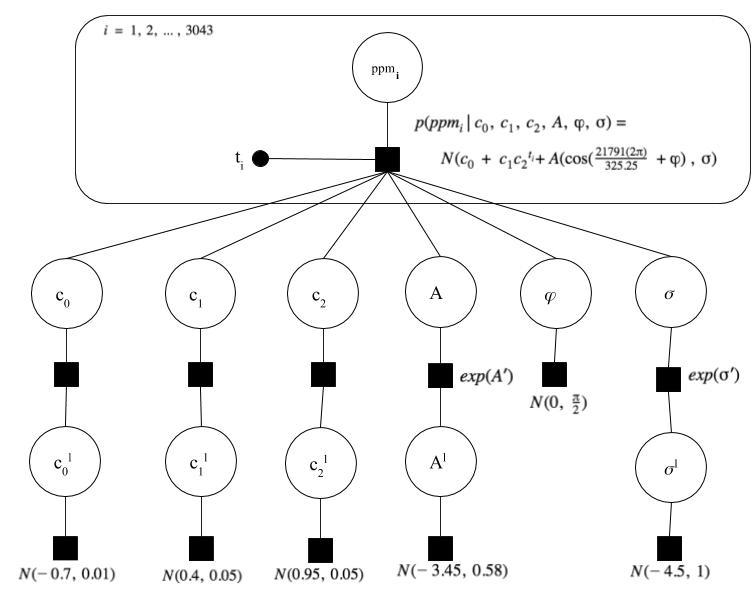
\includegraphics[width=0.8\textwidth]{mauna_loa/exponential_graph.png}
\caption{Exponential likelihood graphical model.}
\end{figure}

\hypertarget{modeling-with-stan}{%
\section{Modeling with Stan}\label{modeling-with-stan}}

I passed the likelihood function and priors to a Stan program, which
uses Hamiltonian Monte Carlo sampling, a form of Markov chain Monte
Carlo sampling, to verge on the underlying distributions for each
parameter. \newline

Both Stan programs converged nicely: all parameters have an
\texttt{Rhat} of 1.0, which means that the ensemble of Markov chains for
each program consistently converged (I used 3 chains per model).

\hypertarget{quadratic-model-sampling-results}{%
\subsection{Quadratic model sampling
results}\label{quadratic-model-sampling-results}}

\begin{longtable}[]{@{}llllllll@{}}
\toprule
Parameter & mean & se\_mean & sd & 5\% & 95\% & eff. sample size &
Rhat\tabularnewline
\midrule
\endhead
c0 & 0.01 & 0 & 0.00 & 0.01 & 0.01 & 2129 & 1\tabularnewline
c1 & 0.51 & 0 & 0.00 & 0.51 & 0.51 & 1836 & 1\tabularnewline
c2 & 0.43 & 0 & 0.00 & 0.42 & 2.44 & 1855 & 1\tabularnewline
A & 0.03 & 0 & 0.00 & 0.03 & 0.03 & 1907 & 1\tabularnewline
phi & -0.43 & 0 & 0.00 & -0.45 & -0.42 & 2013 & 1\tabularnewline
sigma & 0.01 & 0 & 0.00 & 0.01 & 0.01 & 2079 & 1\tabularnewline
\bottomrule
\end{longtable}

\hypertarget{exponential-model-sampling-results}{%
\subsection{Exponential model sampling
results}\label{exponential-model-sampling-results}}

\begin{longtable}[]{@{}llllllll@{}}
\toprule
Parameter & mean & se\_mean & sd & 5\% & 95\% & eff. sample size &
Rhat\tabularnewline
\midrule
\endhead
c0 & -0.59 & 0 & 0.01 & -0.60 & -0.58 & 983 & 1\tabularnewline
c1 & 0.60 & 0 & 0.00 & 0.59 & 0.61 & 983 & 1\tabularnewline
c2 & 2.60 & 0 & 0.01 & 2.58 & 2.63 & 993 & 1\tabularnewline
A & 0.03 & 0 & 0.00 & 0.03 & 0.03 & 2178 & 1\tabularnewline
phi & -0.43 & 0 & 0.01 & -0.45 & -0.41 & 2160 & 1\tabularnewline
sigma & 0.01 & 0 & 0.00 & 0.01 & 0.01 & 2075 & 1\tabularnewline
\bottomrule
\end{longtable}

We can visualize the sampling quality with an autocorrelation function
for each parameter; for brevity's sake, I only include here the ACFs for
the quadratic model's parameter samples, but those for the exponential
model look much the same. As evidenced below, the samples for each
parameter are uncorrelated.

\begin{figure}
\centering
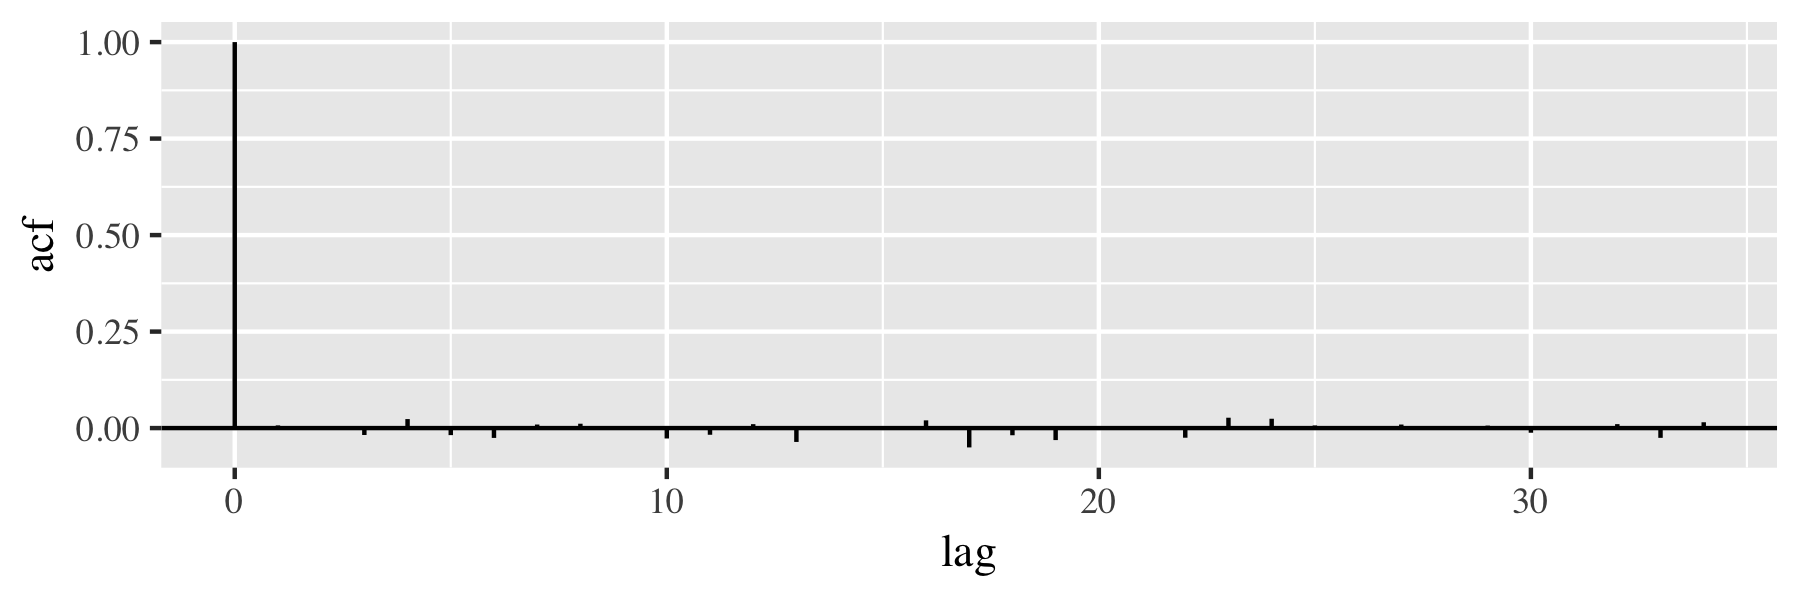
\includegraphics[width=0.55\textwidth]{mauna_loa/auto1.png}
\caption{Autocorrelation of c0 samples}
\end{figure}

\begin{figure}
\centering
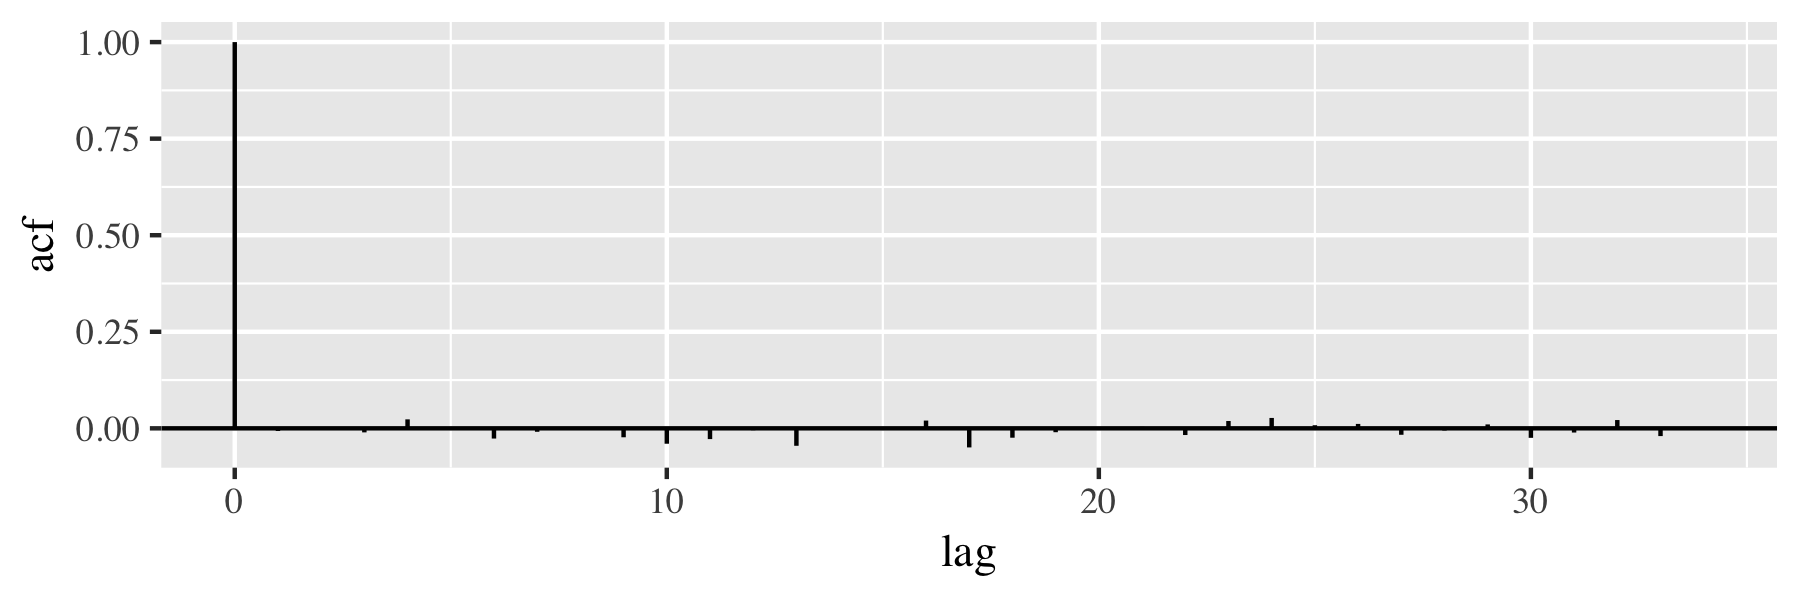
\includegraphics[width=0.55\textwidth]{mauna_loa/auto2.png}
\caption{Autocorrelation of c1 samples}
\end{figure}

\begin{figure}
\centering
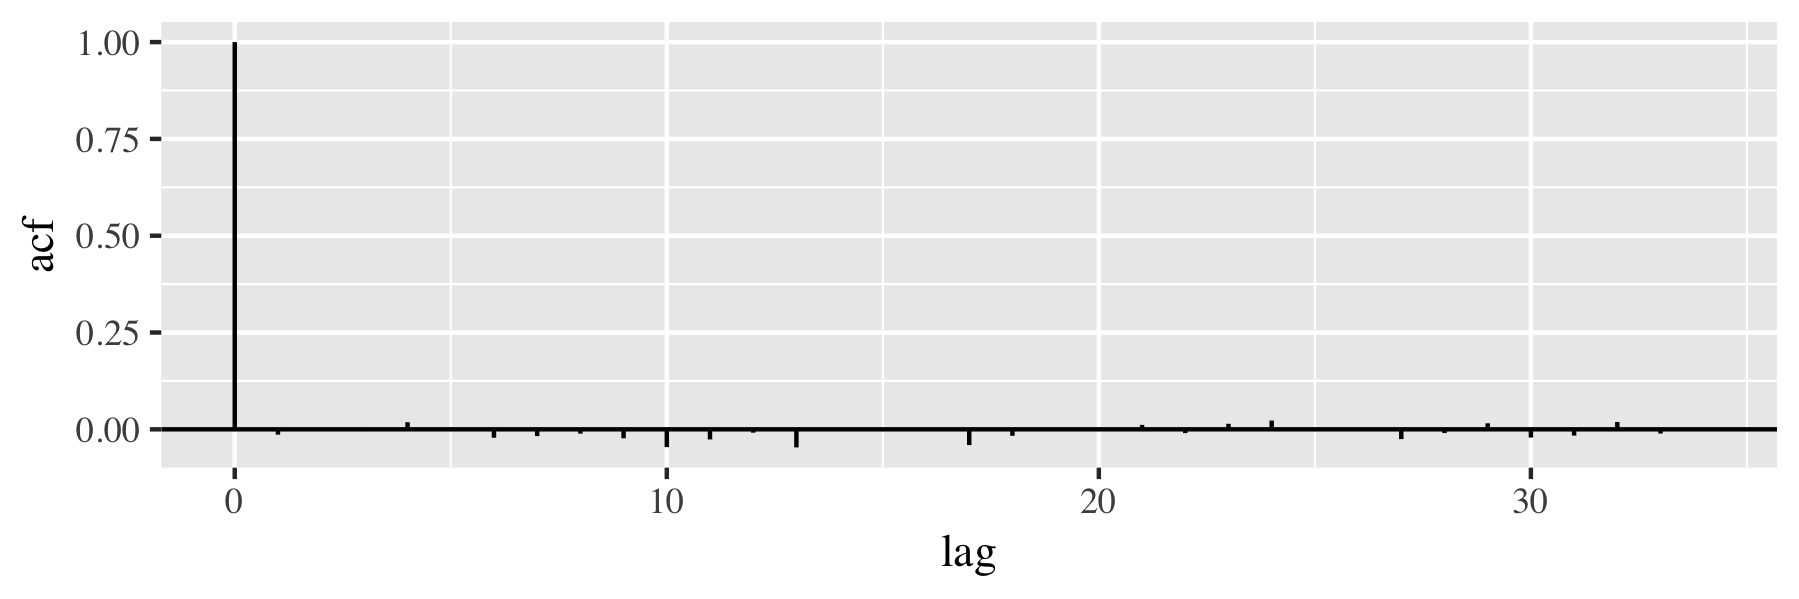
\includegraphics[width=0.55\textwidth]{mauna_loa/auto3.png}
\caption{Autocorrelation of c2 samples}
\end{figure}

\begin{figure}
\centering
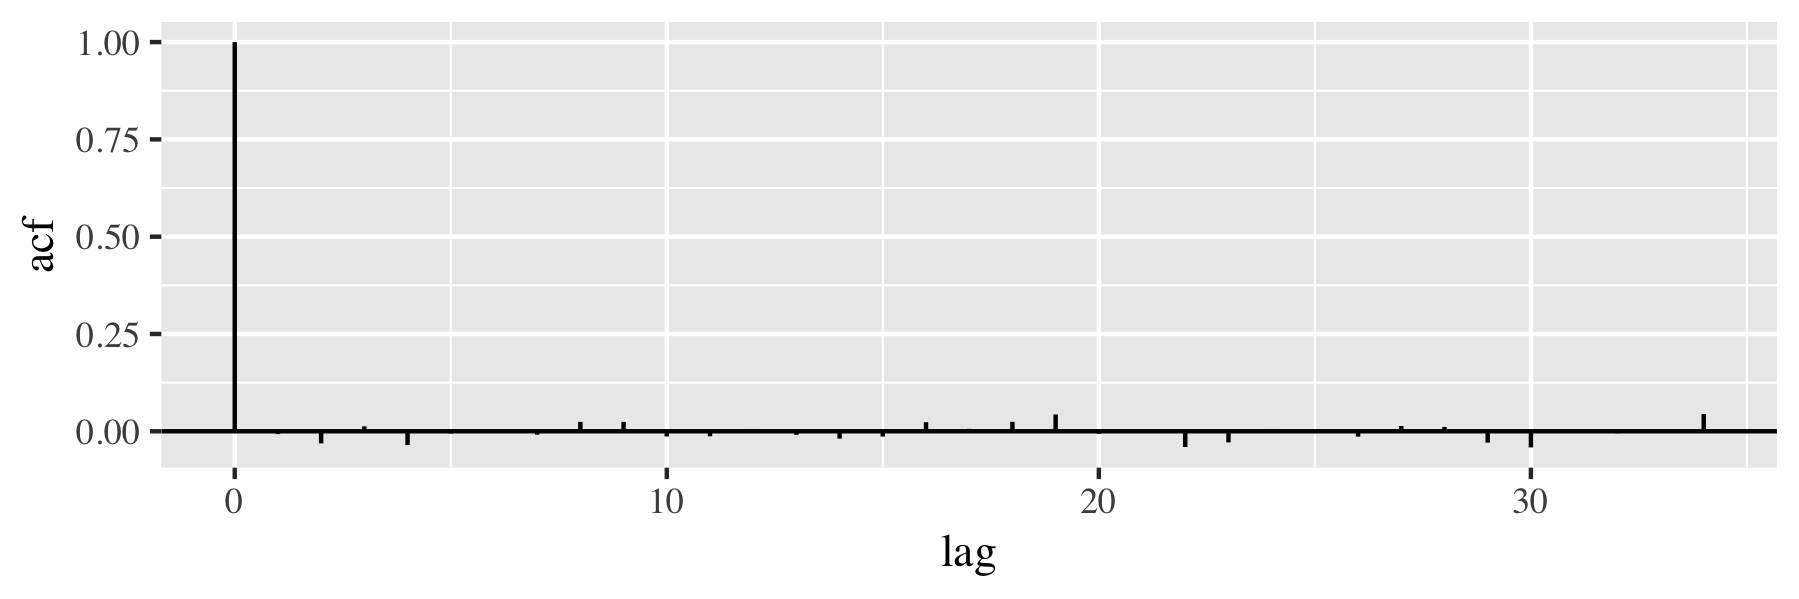
\includegraphics[width=0.55\textwidth]{mauna_loa/auto4.png}
\caption{``Autocorrelation of A samples''}
\end{figure}

\begin{figure}
\centering
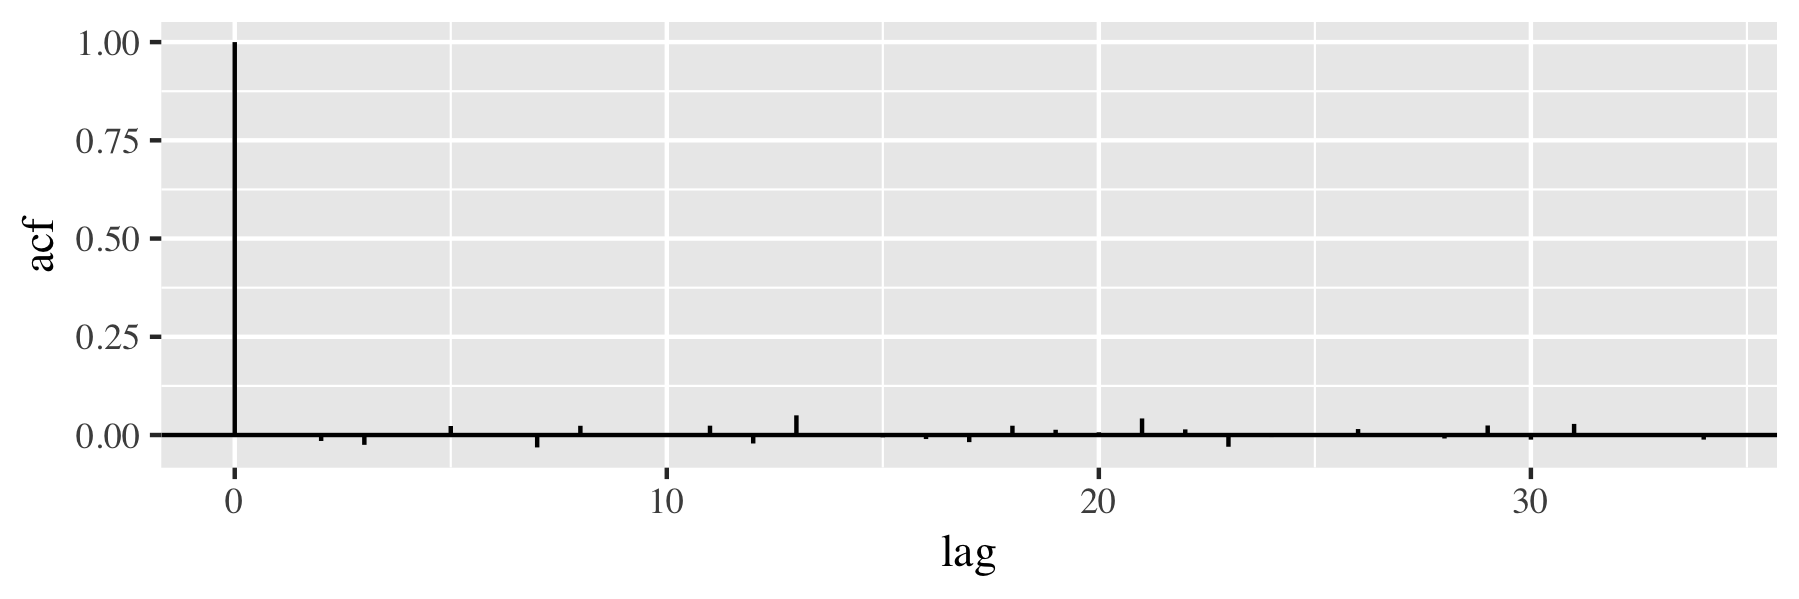
\includegraphics[width=0.55\textwidth]{mauna_loa/auto5.png}
\caption{Autocorrelation of phi samples}
\end{figure}

\begin{figure}
\centering
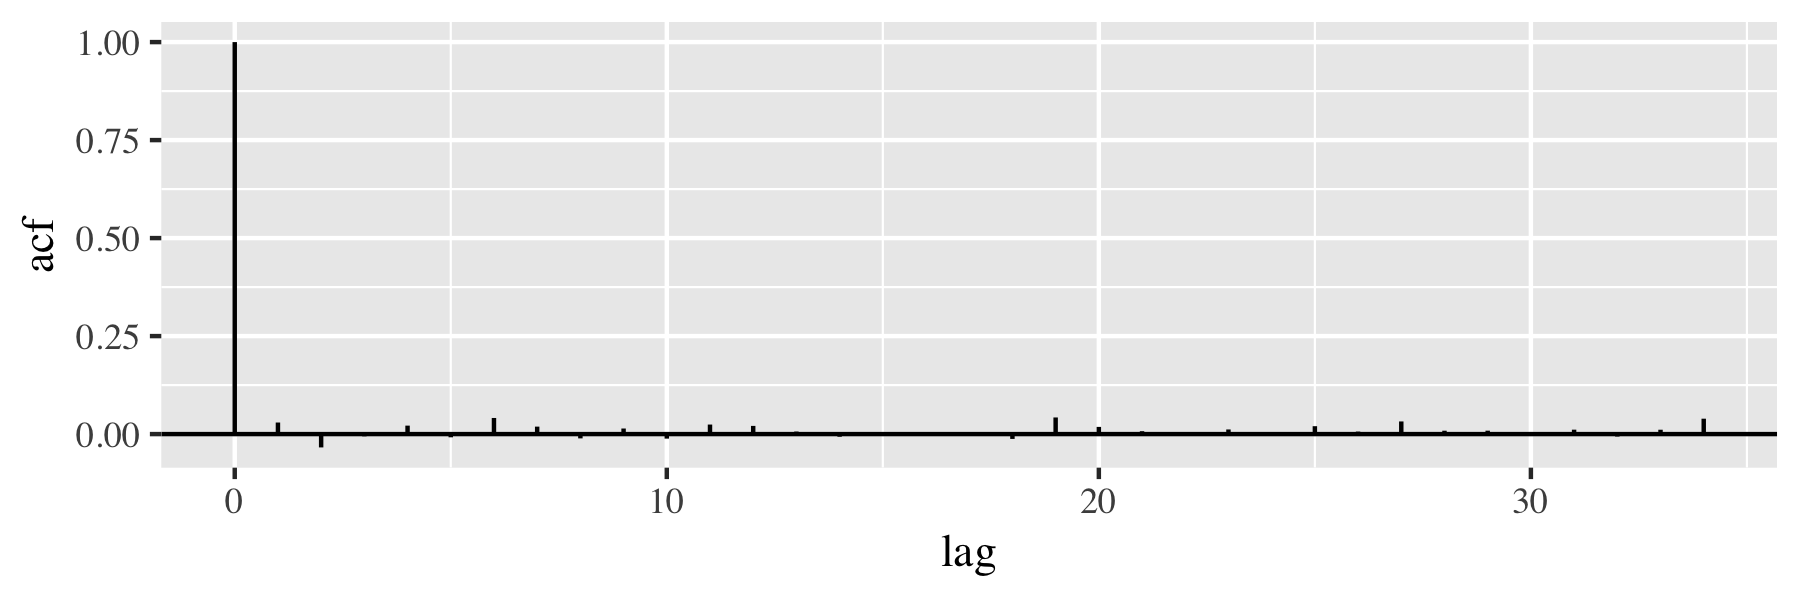
\includegraphics[width=0.55\textwidth]{mauna_loa/auto6.png}
\caption{Autocorrelation of sigma samples}
\end{figure}

Finally, we see the 95\% confidence intervals over the posterior
predicted samples for the training dates (1958-2006) and test dates
(2006-2017).

\begin{figure}
\centering
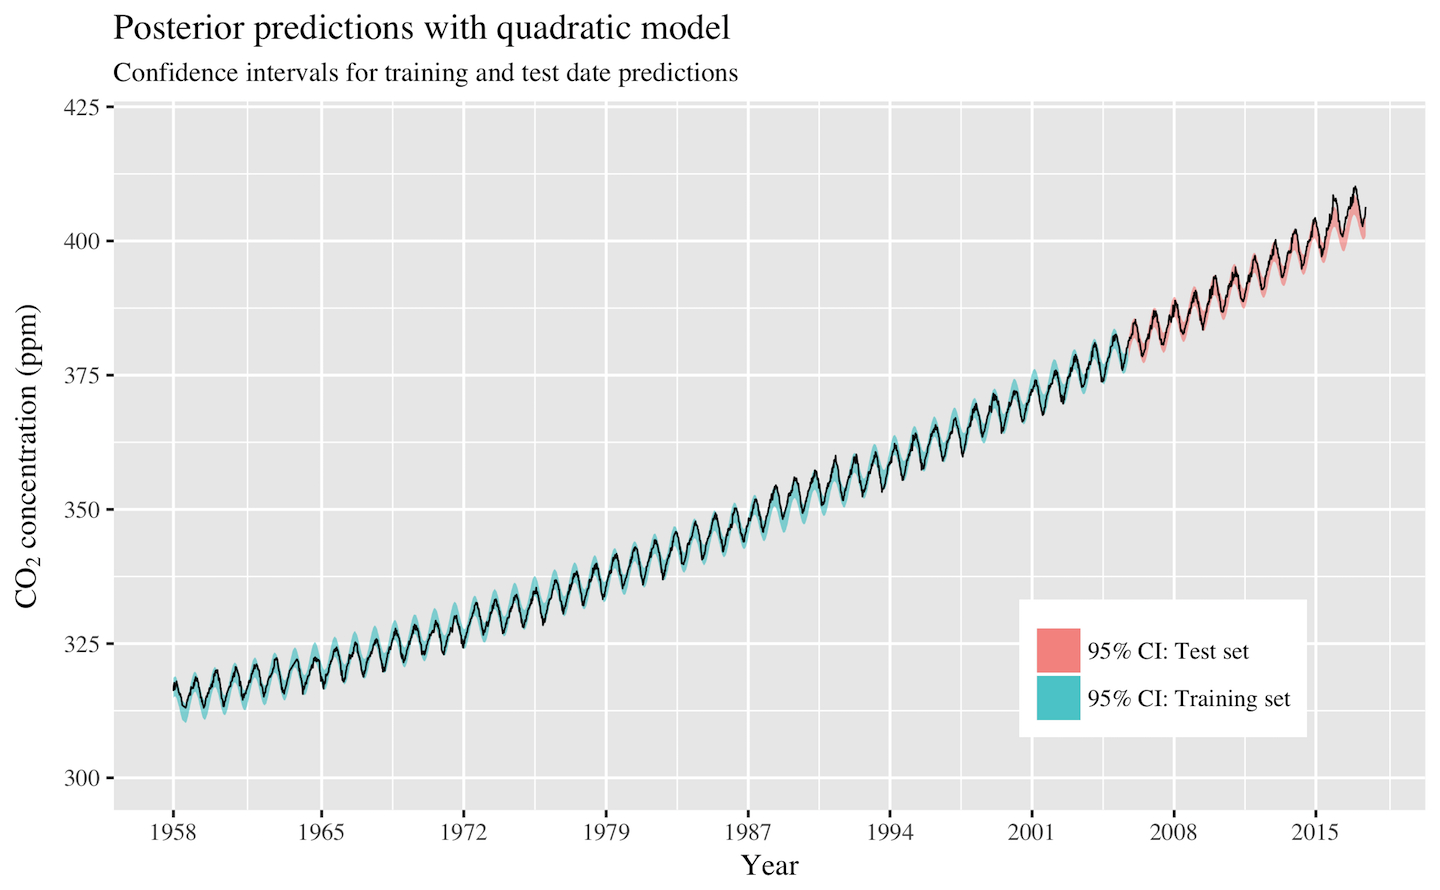
\includegraphics[width=0.7\textwidth]{mauna_loa/quad_intervals.png}
\caption{Quadratic model posterior sampling}
\end{figure}

\begin{figure}
\centering
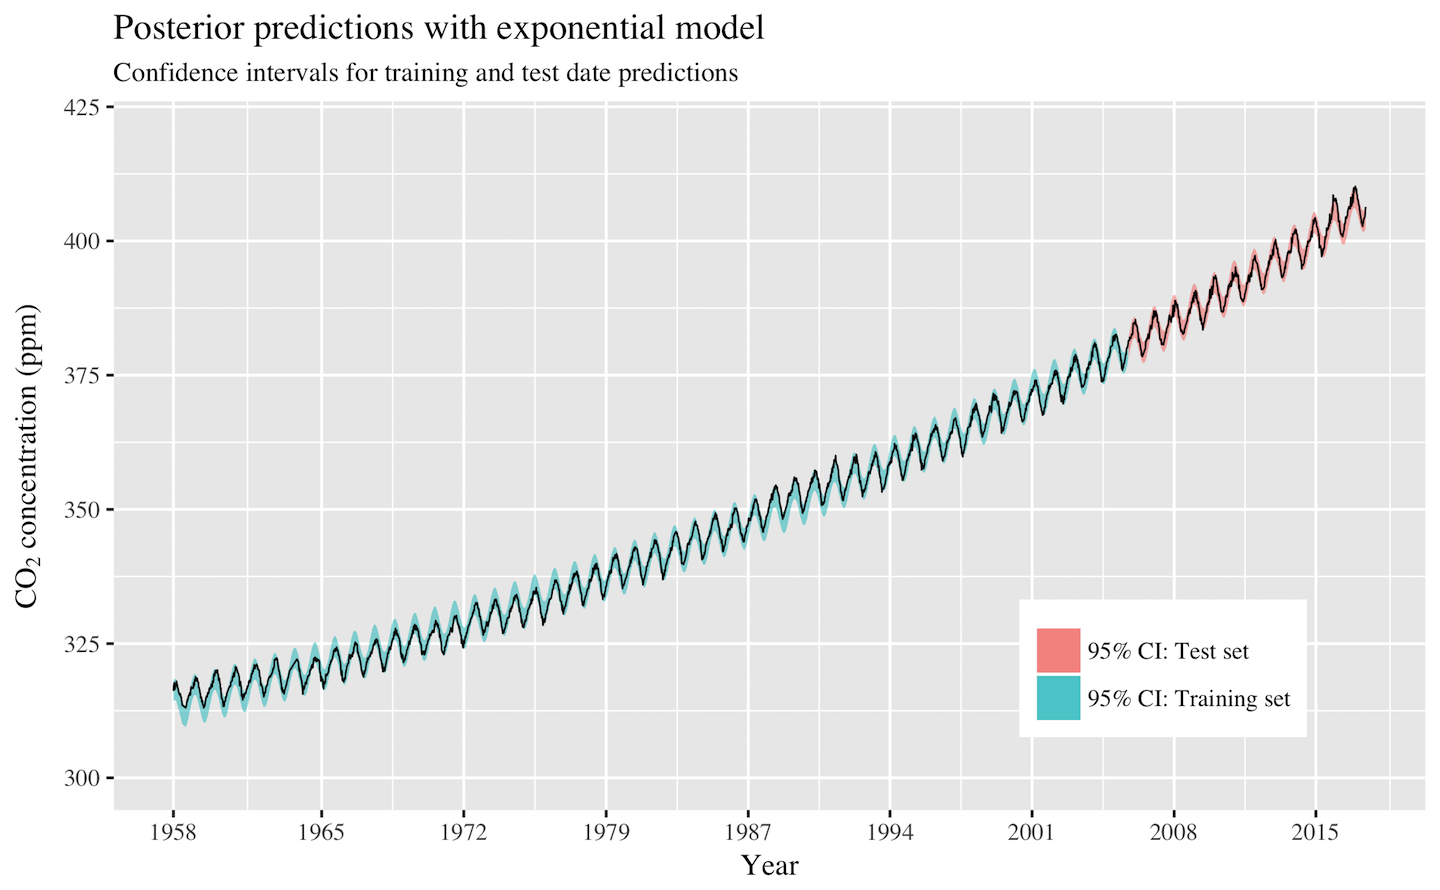
\includegraphics[width=0.7\textwidth]{mauna_loa/exp_intervals.png}
\caption{Exponential model posterior sampling}
\end{figure}

The quadratic model has a root mean square error (RMSE) of 1.32 on the
test set, whereas the exponential model has only 0.91. But furthermore,
I'm interested in the marginal likelihood of the data, given each model.
I used the \texttt{bridgesampling} package to compute the (log) marginal
likelihood of each model, re-fitting with \texttt{Stan} on the
\emph{full} dataset (as the marginal likelihood represents how well the
fit explains \emph{all}, as opposed to some of the data, I don't want to
lose the information contained in the test set dates). \newline

Analysis with \texttt{bridgesampling} suggests that the estimated Bayes
factor --- which quantifies the evidence for one hypothesis over another
--- in favor of the quadratic model over the exponential is equal to
3.094133e+22. I tend to prefer the exponential one, because its forecast
suits my pessimism (it nearly hits 550 ppm by 2058):\newline

\begin{figure}
\centering
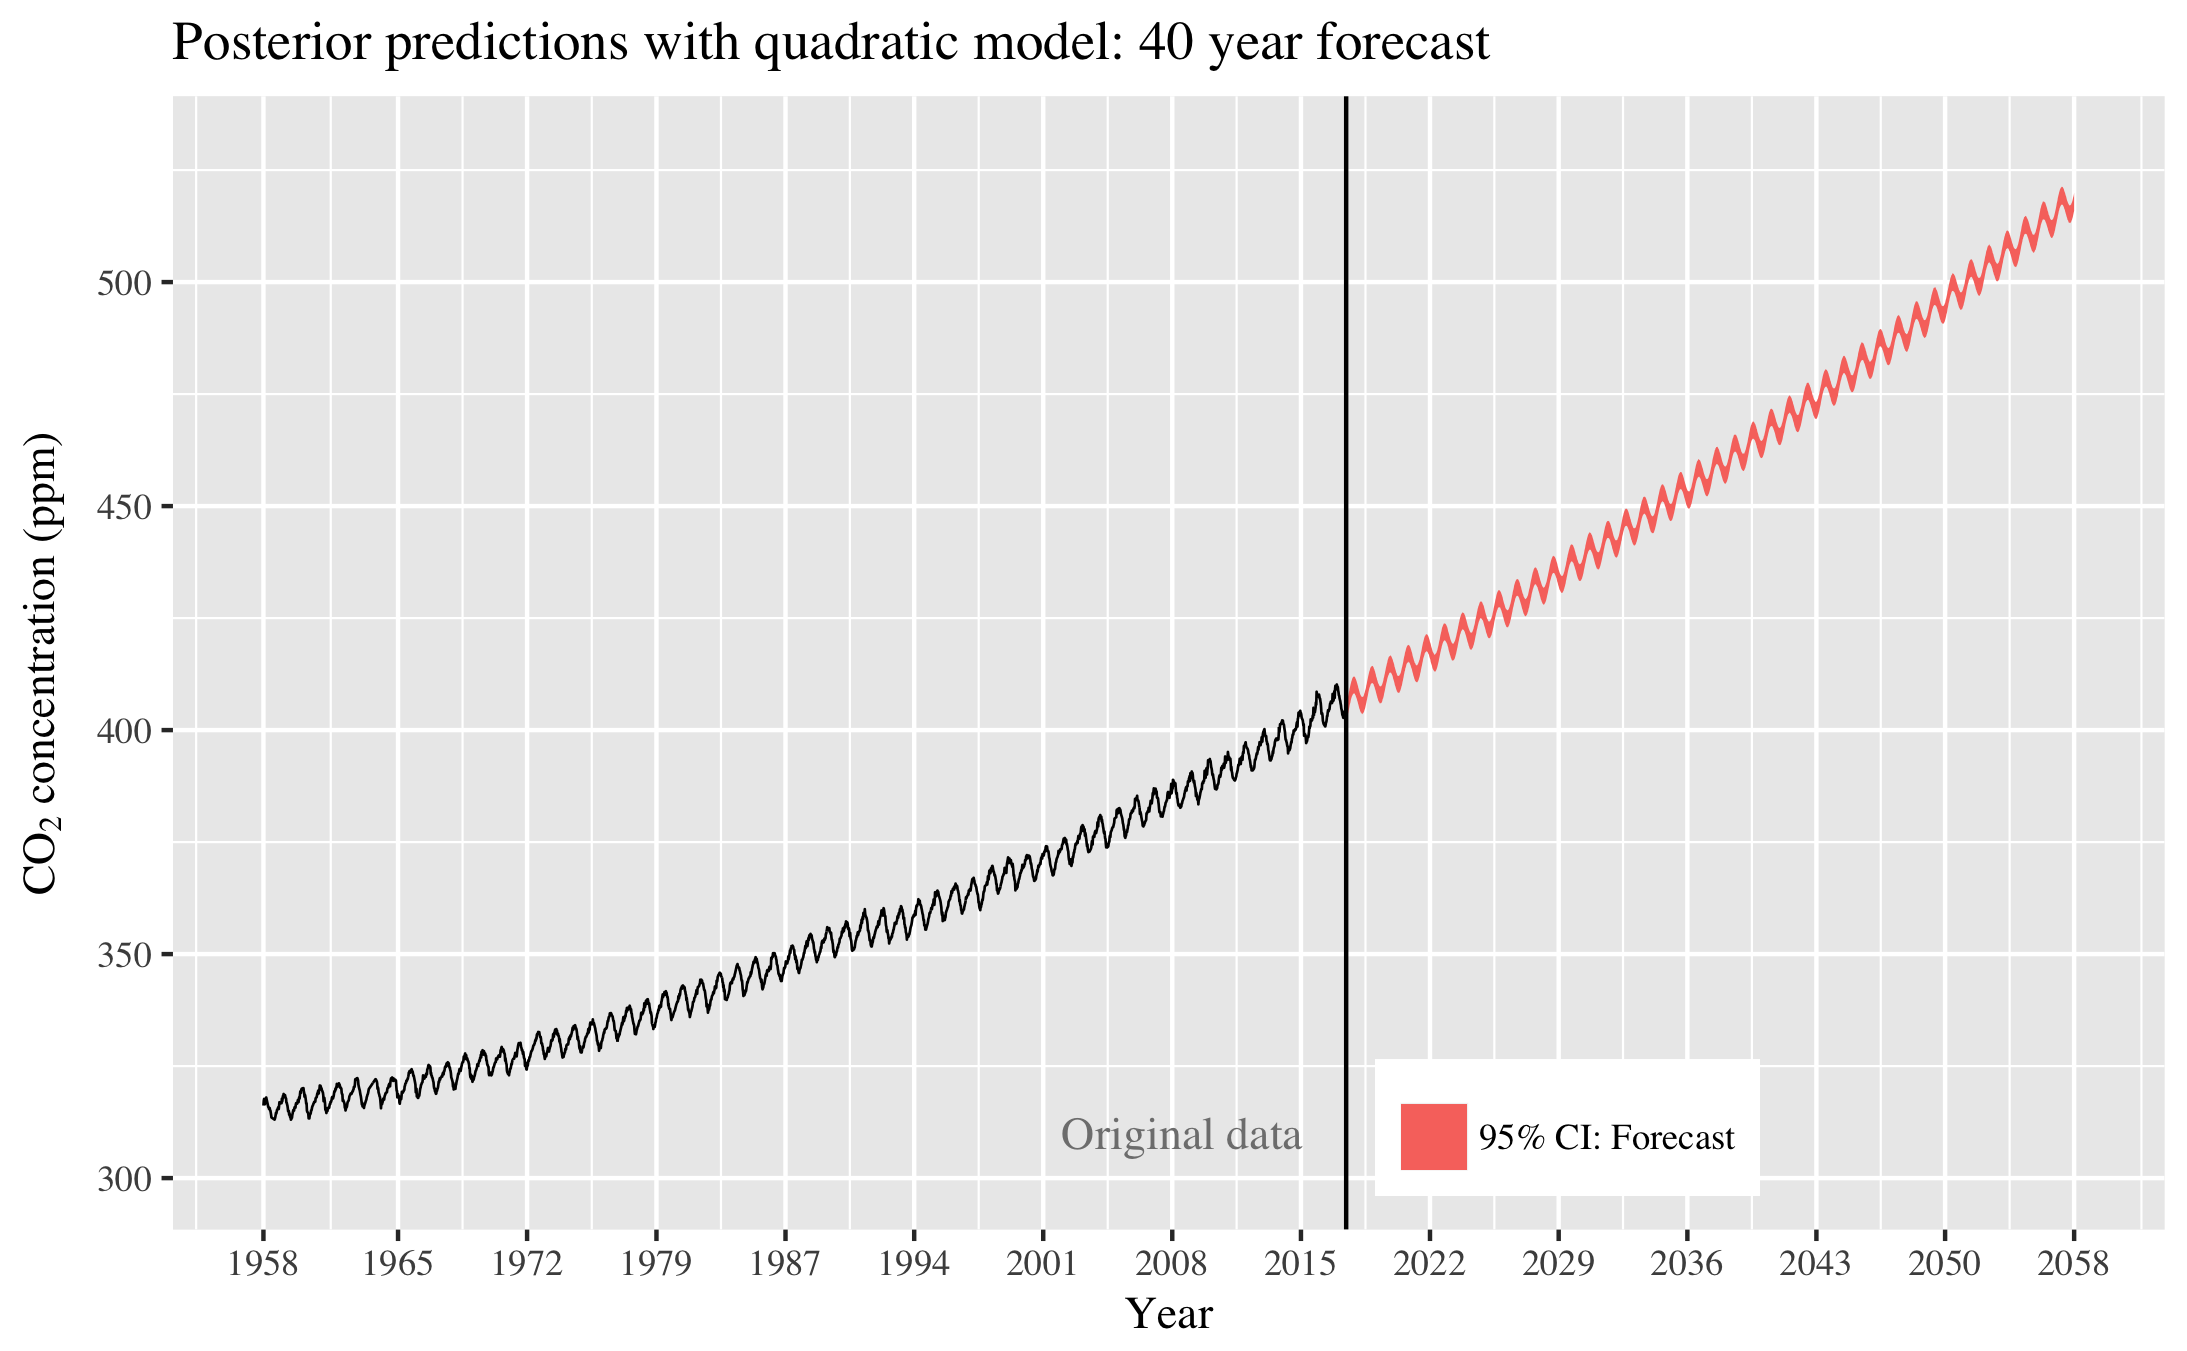
\includegraphics[width=0.7\textwidth]{mauna_loa/quad_forecast.png}
\caption{Quadratic forecast}
\end{figure}

\begin{figure}
\centering
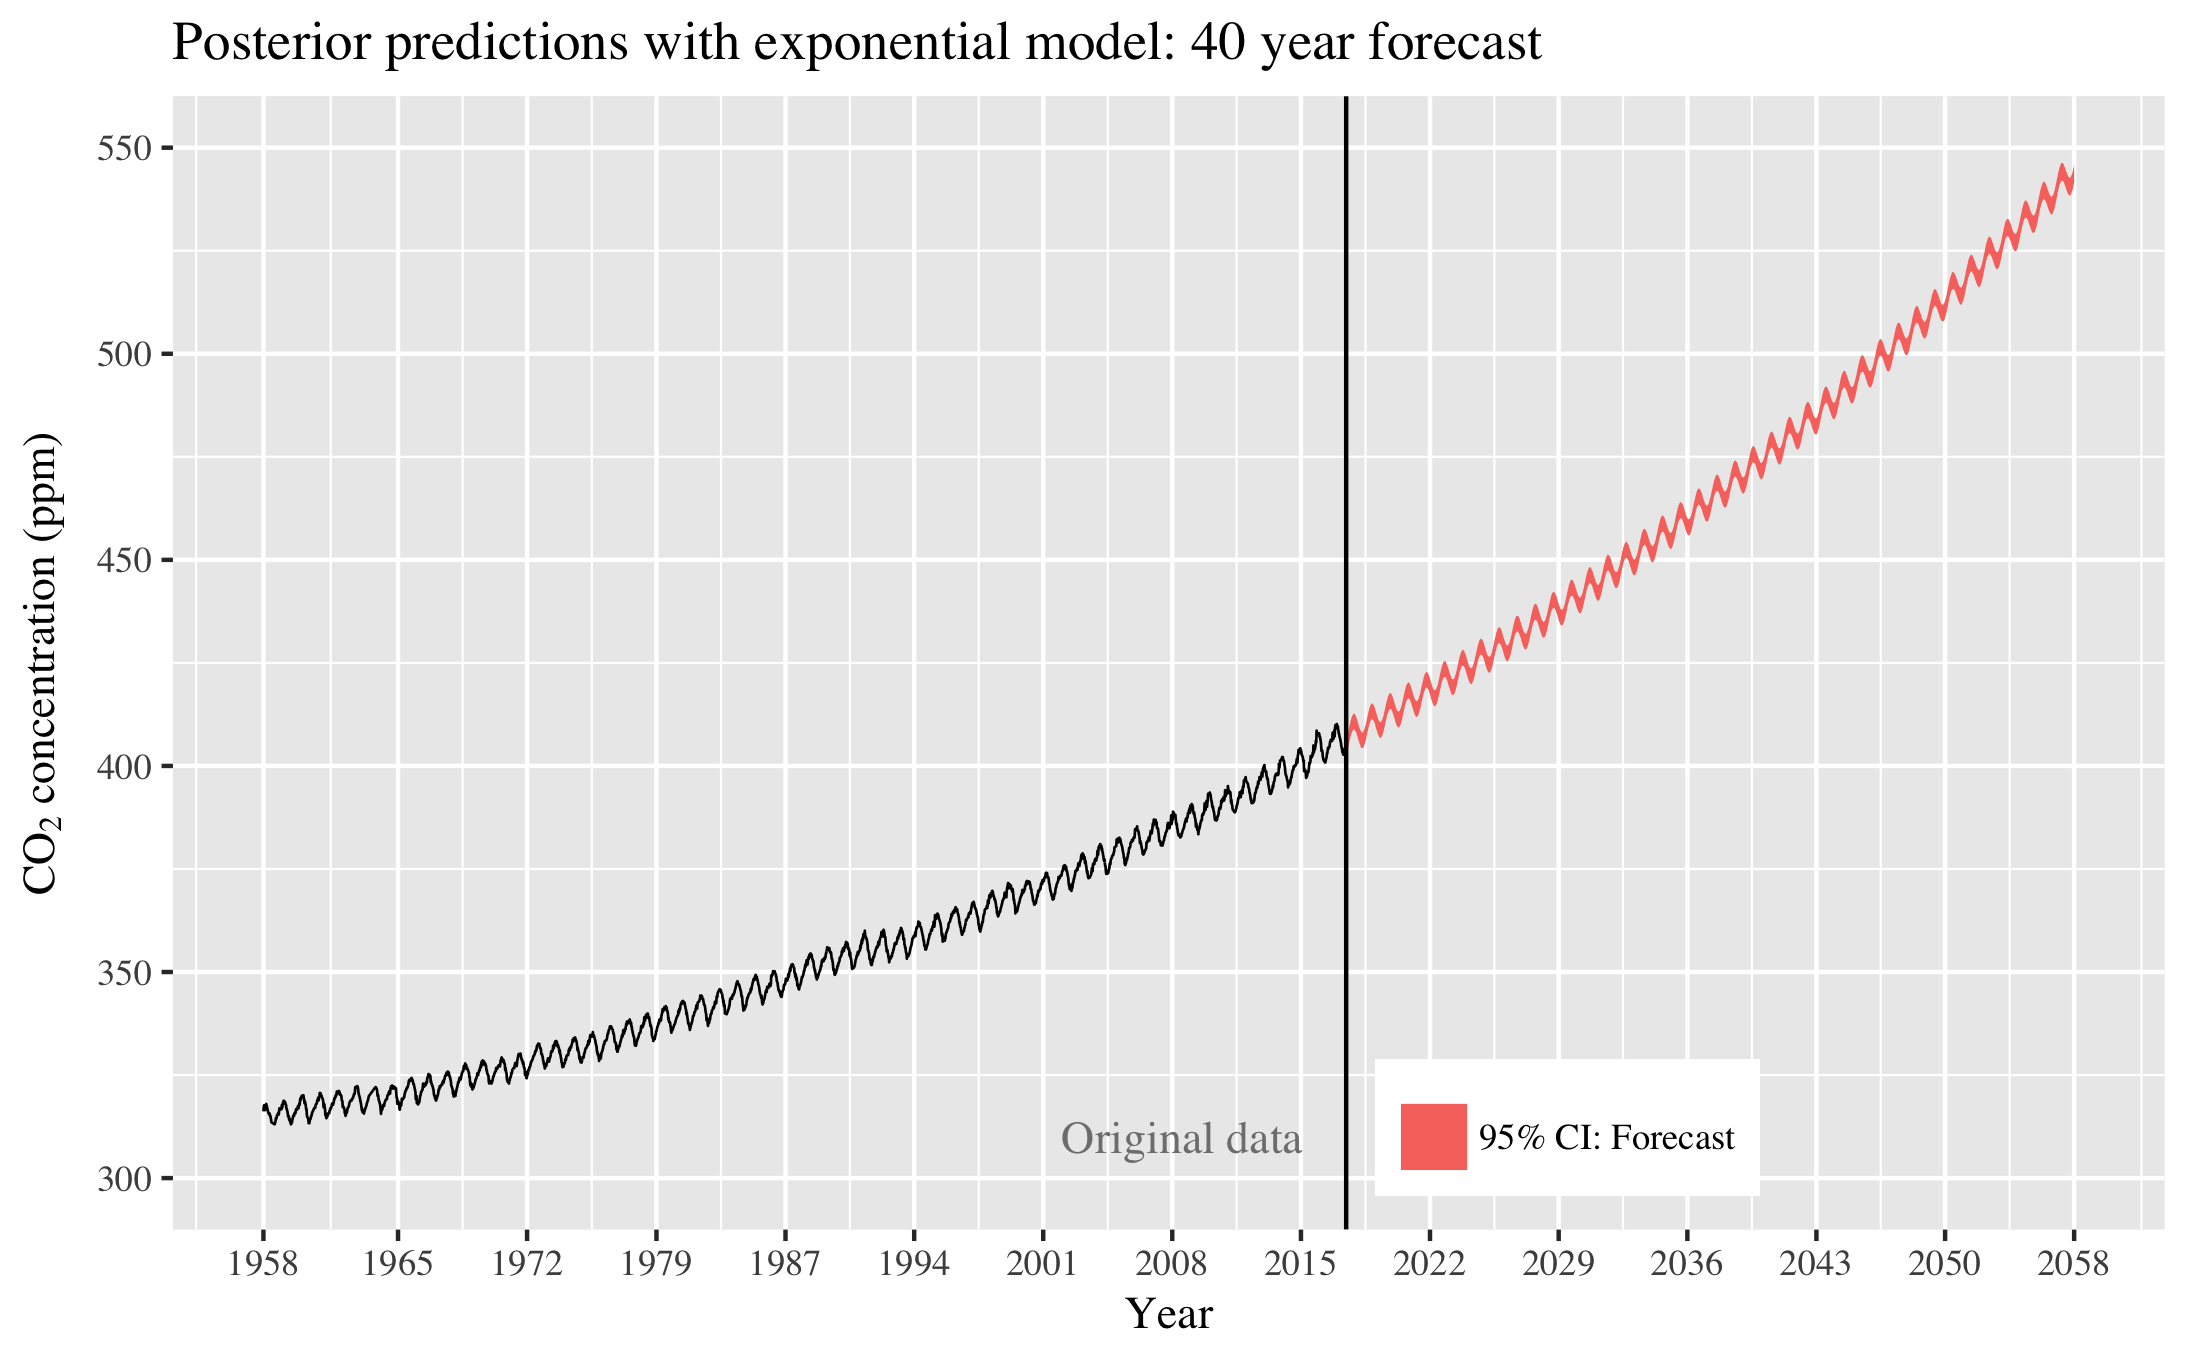
\includegraphics[width=0.7\textwidth]{mauna_loa/exp_forecast.png}
\caption{Exponential forecast}
\end{figure}

But considering the higher marginal likelihood with the quadratic model,
I make the following predictions using that one.

\hypertarget{predictions}{%
\section{Predictions}\label{predictions}}

On January 5th, 2058, the 95\% confidence interval for atmospheric
CO\(_2\) has a lower bound of \textbf{516.0349} ppm, and an upper bound
of \textbf{519.9429} ppm. Furthermore, the 95\% confidence interval
bounds 450 ppm at the dates February 18th, 2034, and March 17th, 2035.
Formally, this means that in 100 experiments with the same amount of
samples, we could expect 95 to contain the true value in their
confidence intervals. Colloquially, it means that the year of 2034 is
looking pretty dangerous: once we hit 450 ppm, we critically diminish
our chance at limiting global warming to 2 degrees Celsius.

\begin{figure}
\centering
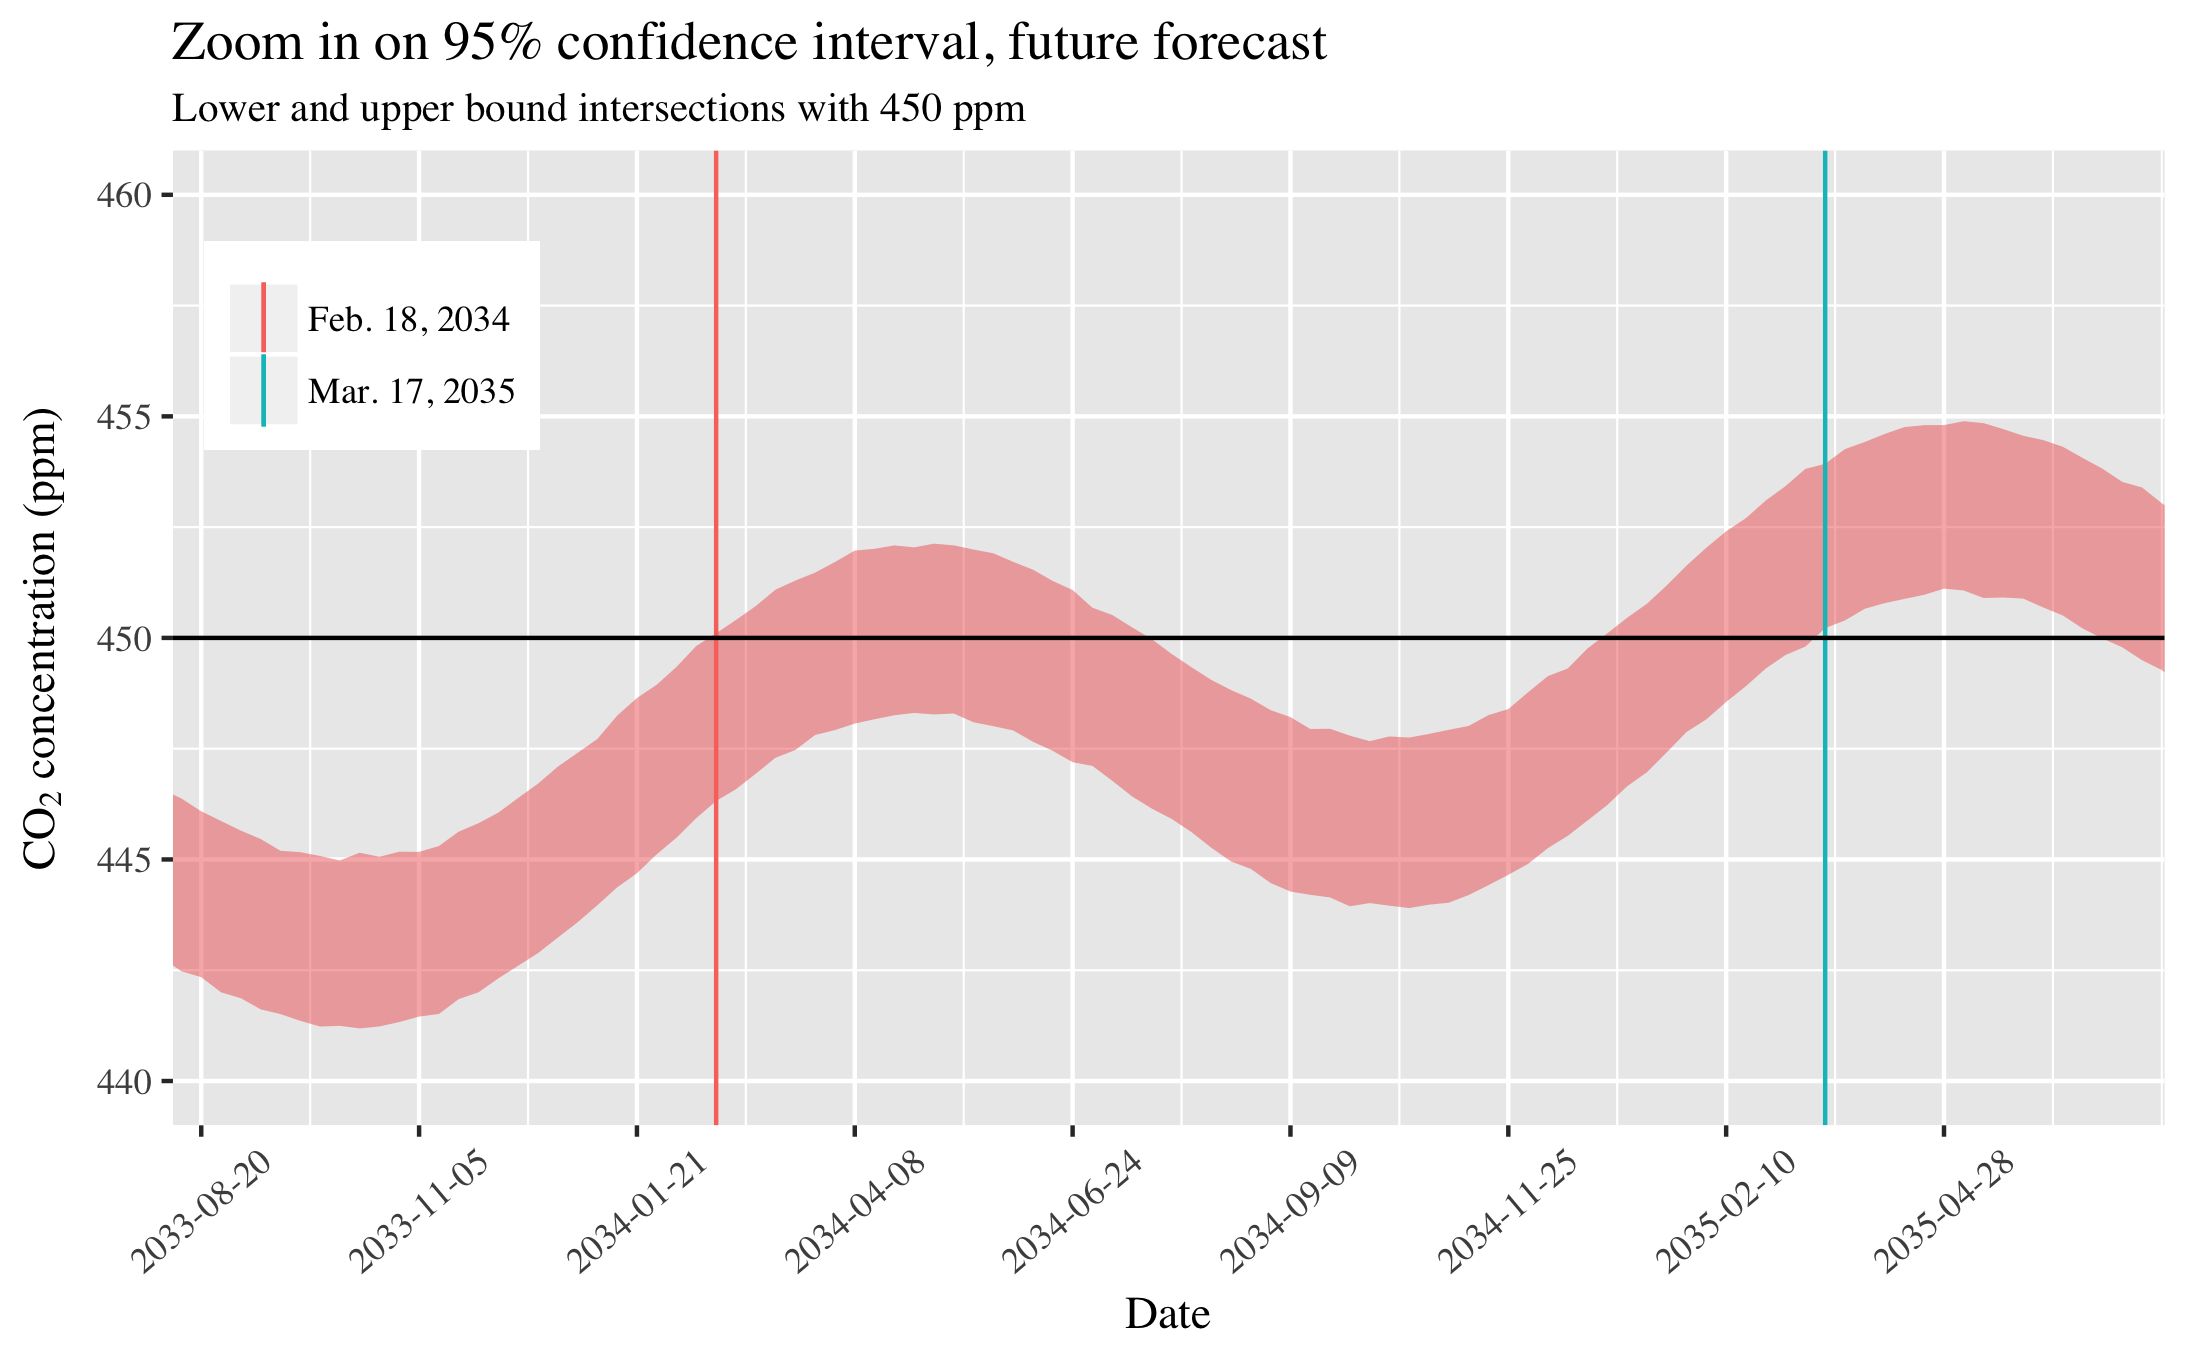
\includegraphics[width=0.8\textwidth]{mauna_loa/zoom-in.png}
\caption{Upper and lower confidence bounds, 450 ppm}
\end{figure}




\newpage
\singlespacing 
\end{document}
